\documentclass{article}
\usepackage{graphicx} % Required for inserting images
\usepackage{booktabs}
\usepackage{multirow}
\usepackage{xcolor}
\usepackage{adjustbox}
\usepackage{subcaption}

\newcommand{\red}[1]{{\color{red}#1}}

\title{Mistat bootstrap analysis}
\author{Peter Gedeck}
\date{August 2023}



\begin{document}

\maketitle

\section{Bootstrap approaches}
\begin{description}
    \item[Bootstrap Analysis (BA):] For each resample, create a new dataset by randomly sampling rows from the original dataset with replacement
    \item[Befitting Bootstrap Analysis (BBA):] For each resample, create a new dataset by randomly sampling rows from each group with replacement
    \item[Parametric Bootstrap Analysis (pBA):] Create a model using the original dataset. For each resample, replace the outcome with adding randomly sampled residuals (with replacement) to the predicted values from the original model.
    \item[Parametric Befitting Bootstrap Analysis (pBBA):] For each resample, replace the outcome values for each group with a random values sampled from a normal distribution with mean and standard deviation as the original group.
    \item[Wild Bootstrap Analysis (wBA):] Create a model using the original dataset. For each resample, multiply the residuals with a random value sampled from a normal distribution $N(0,1)$ and add to the fitted values from the original model.
\end{description}

\section{Wave soldering dataset}
\begin{figure}
    \centering
    \begin{subfigure}[c]{\textwidth}
        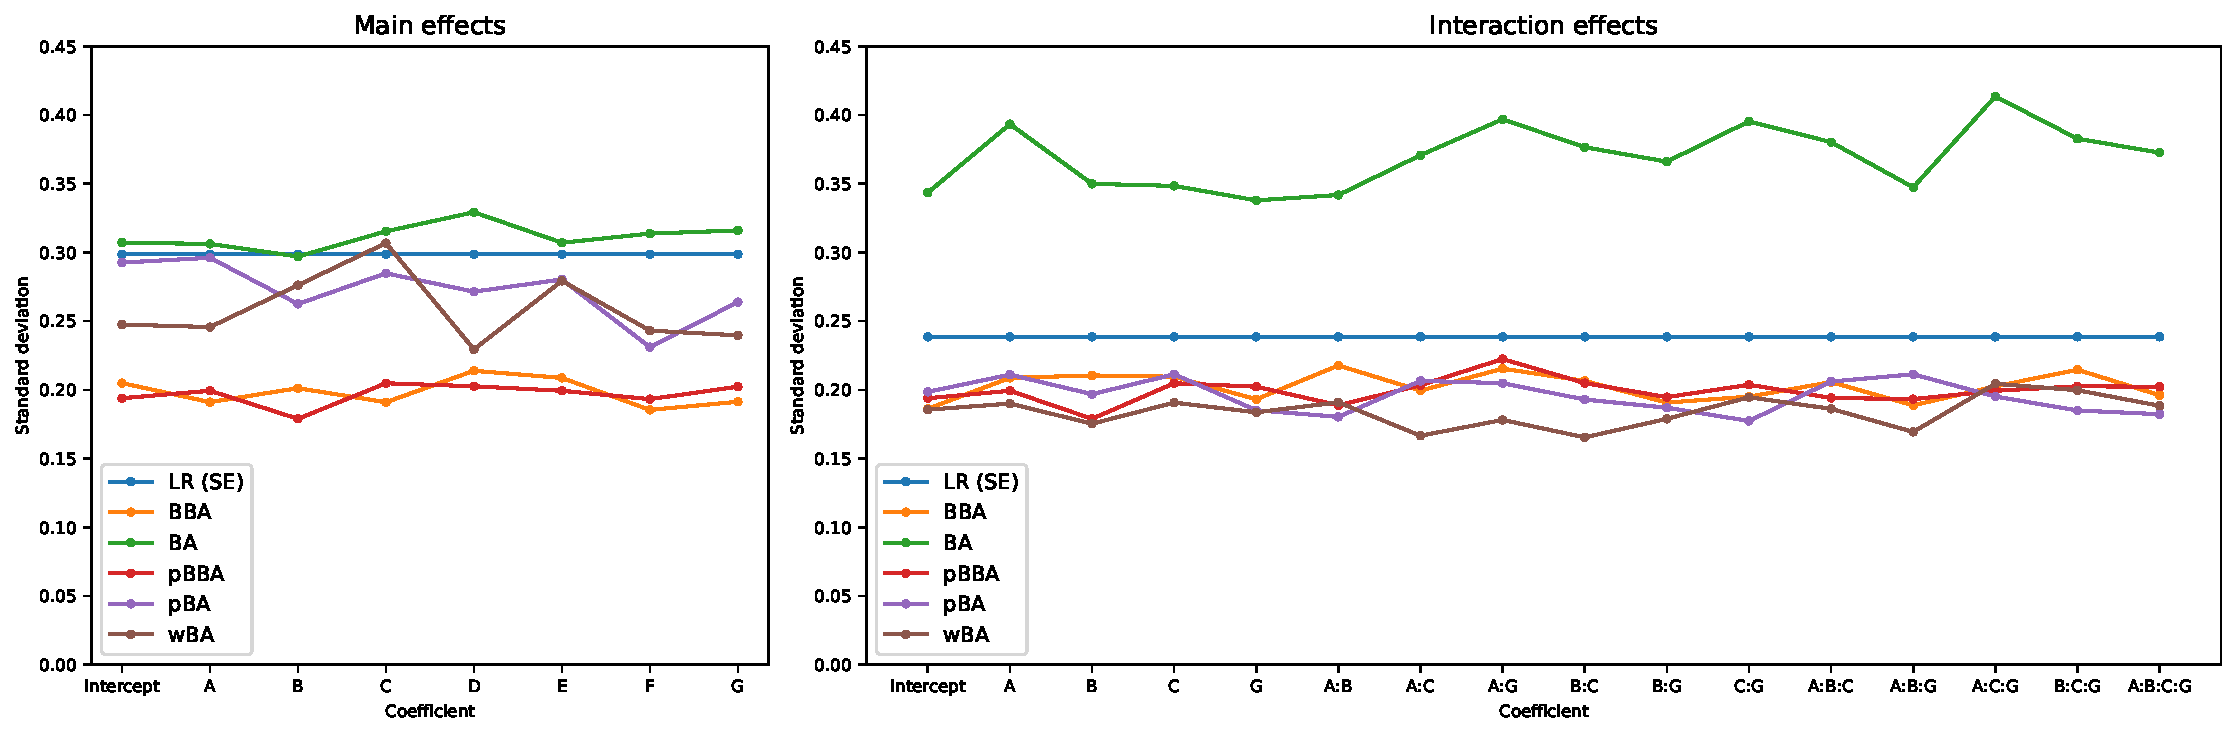
\includegraphics[width=\linewidth]{figures/wavesoldering-std.pdf}
        \caption{100 bootstrap samples}
        \label{fig:wavesoldering-std-100}
    \end{subfigure}
    \begin{subfigure}[c]{\textwidth}
        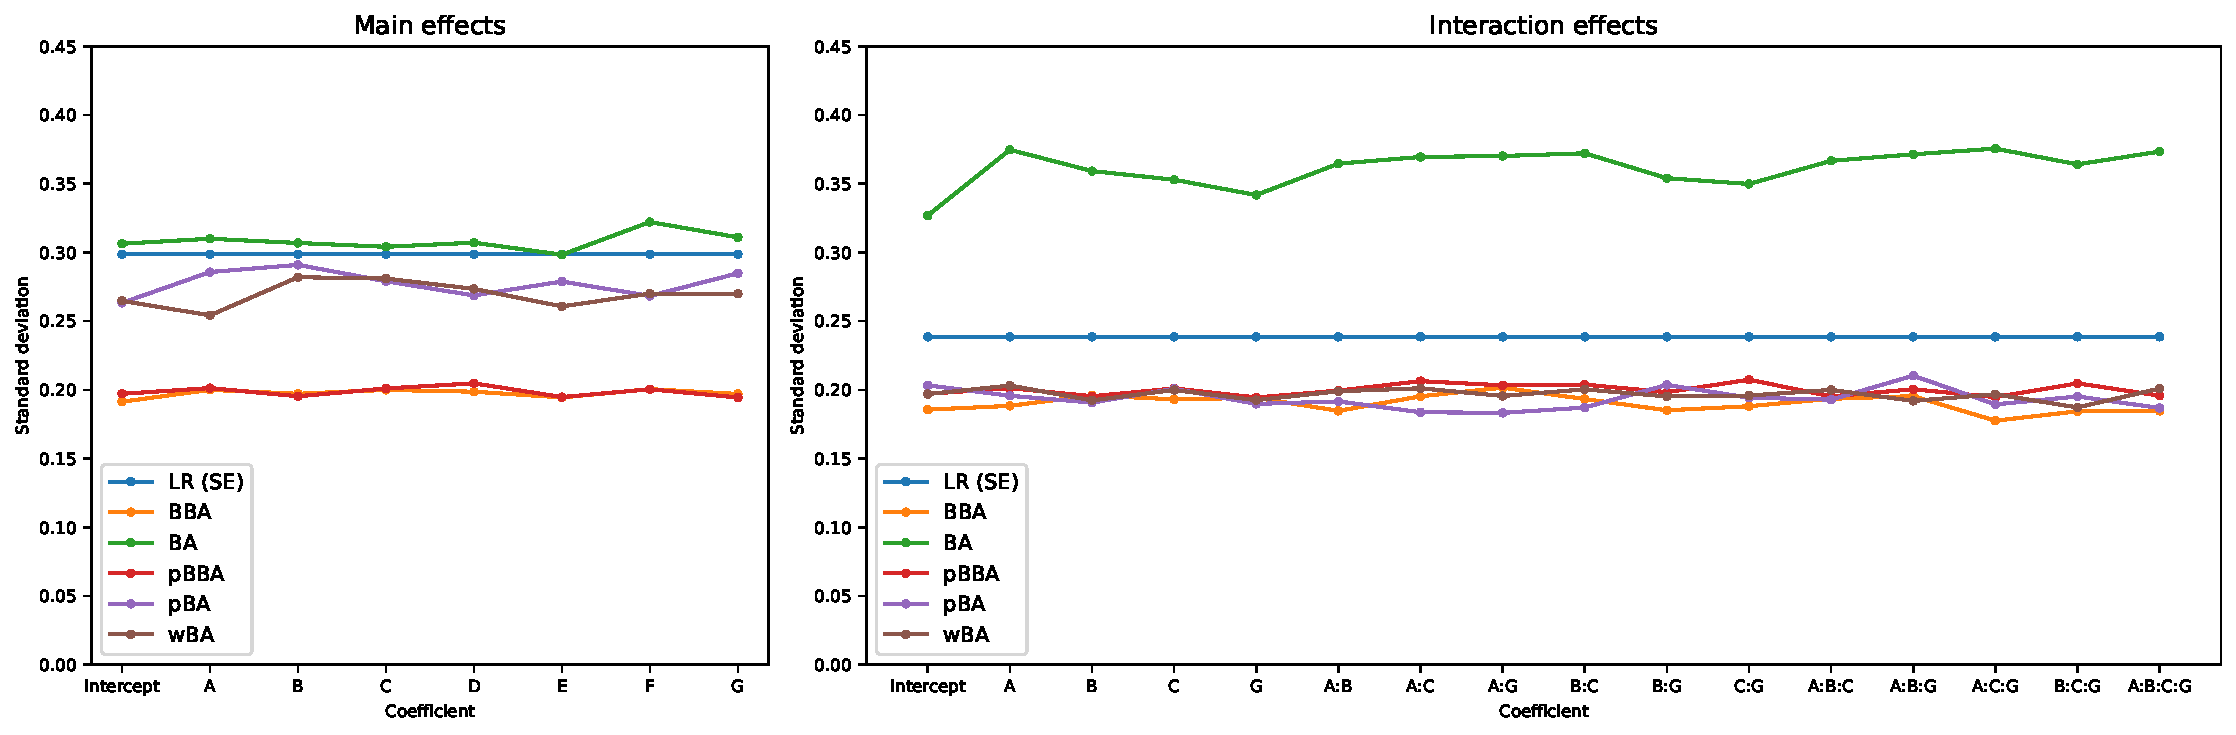
\includegraphics[width=\linewidth]{figures/wavesoldering-std-500.pdf}
        \caption{500 bootstrap samples}
        \label{fig:wavesoldering-std-500}
    \end{subfigure}
    \begin{subfigure}[c]{\textwidth}
        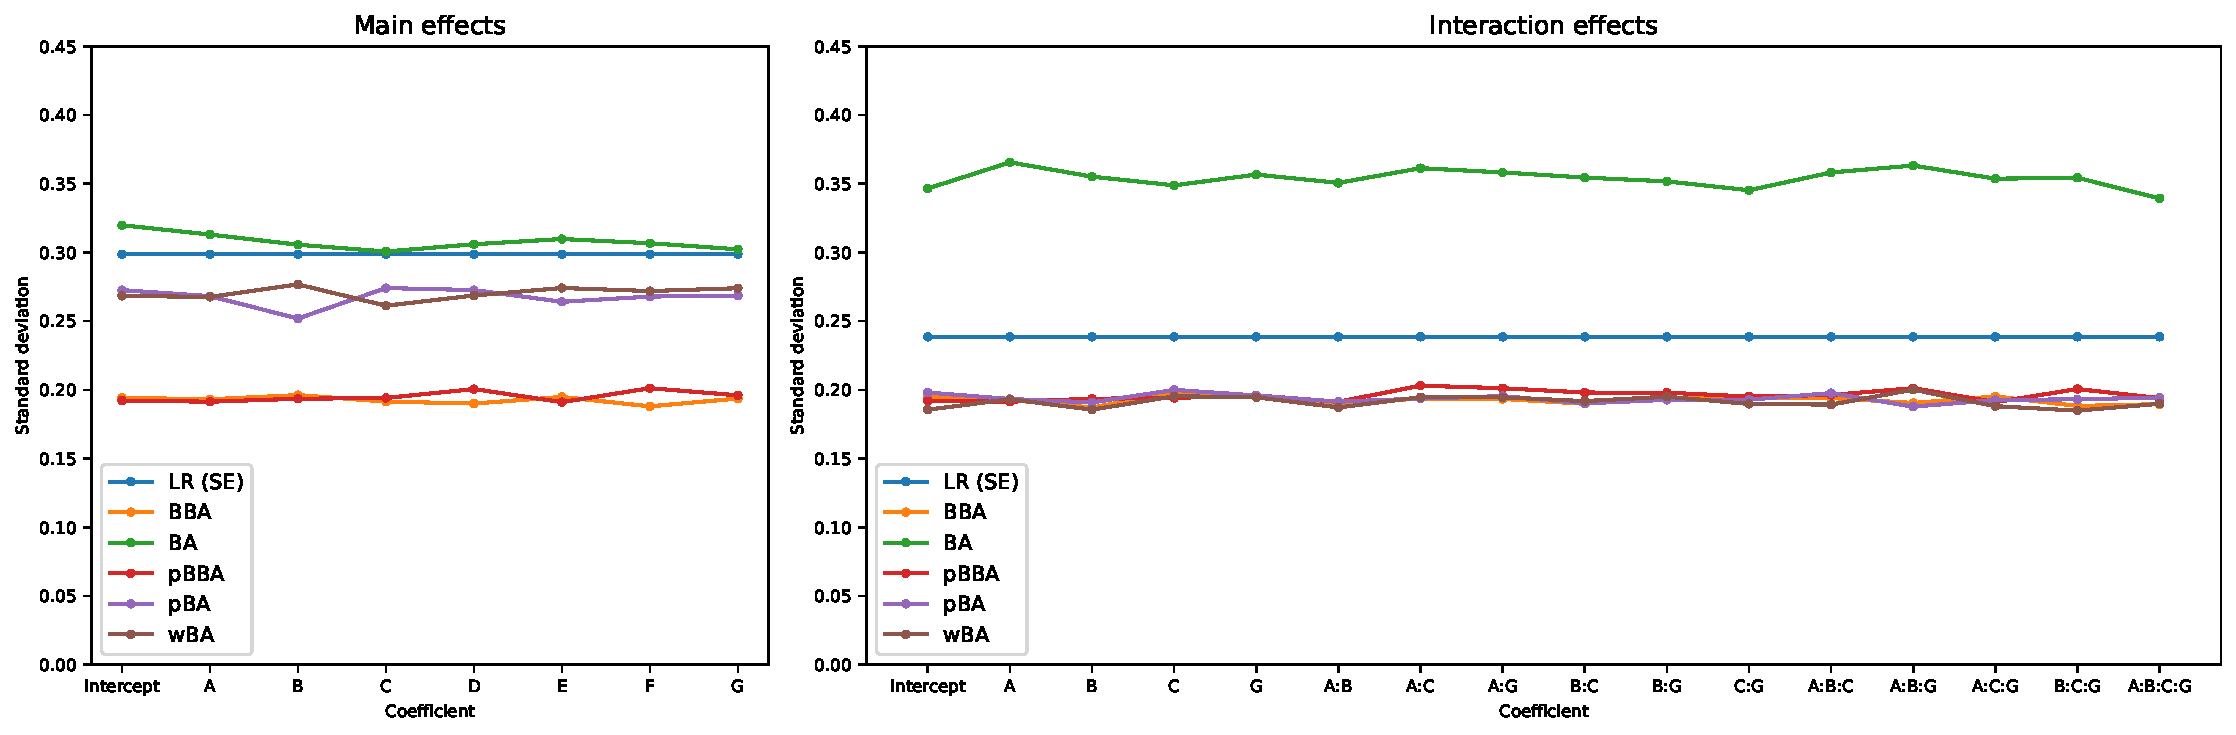
\includegraphics[width=\linewidth]{figures/wavesoldering-std-1000.pdf}
        \caption{1000 bootstrap samples}
        \label{fig:wavesoldering-std-1000}
    \end{subfigure}
    \caption{Std.dev. of coefficients for wave soldering dataset}
    \label{fig:wavesoldering-std}
\end{figure}
\begin{figure}
    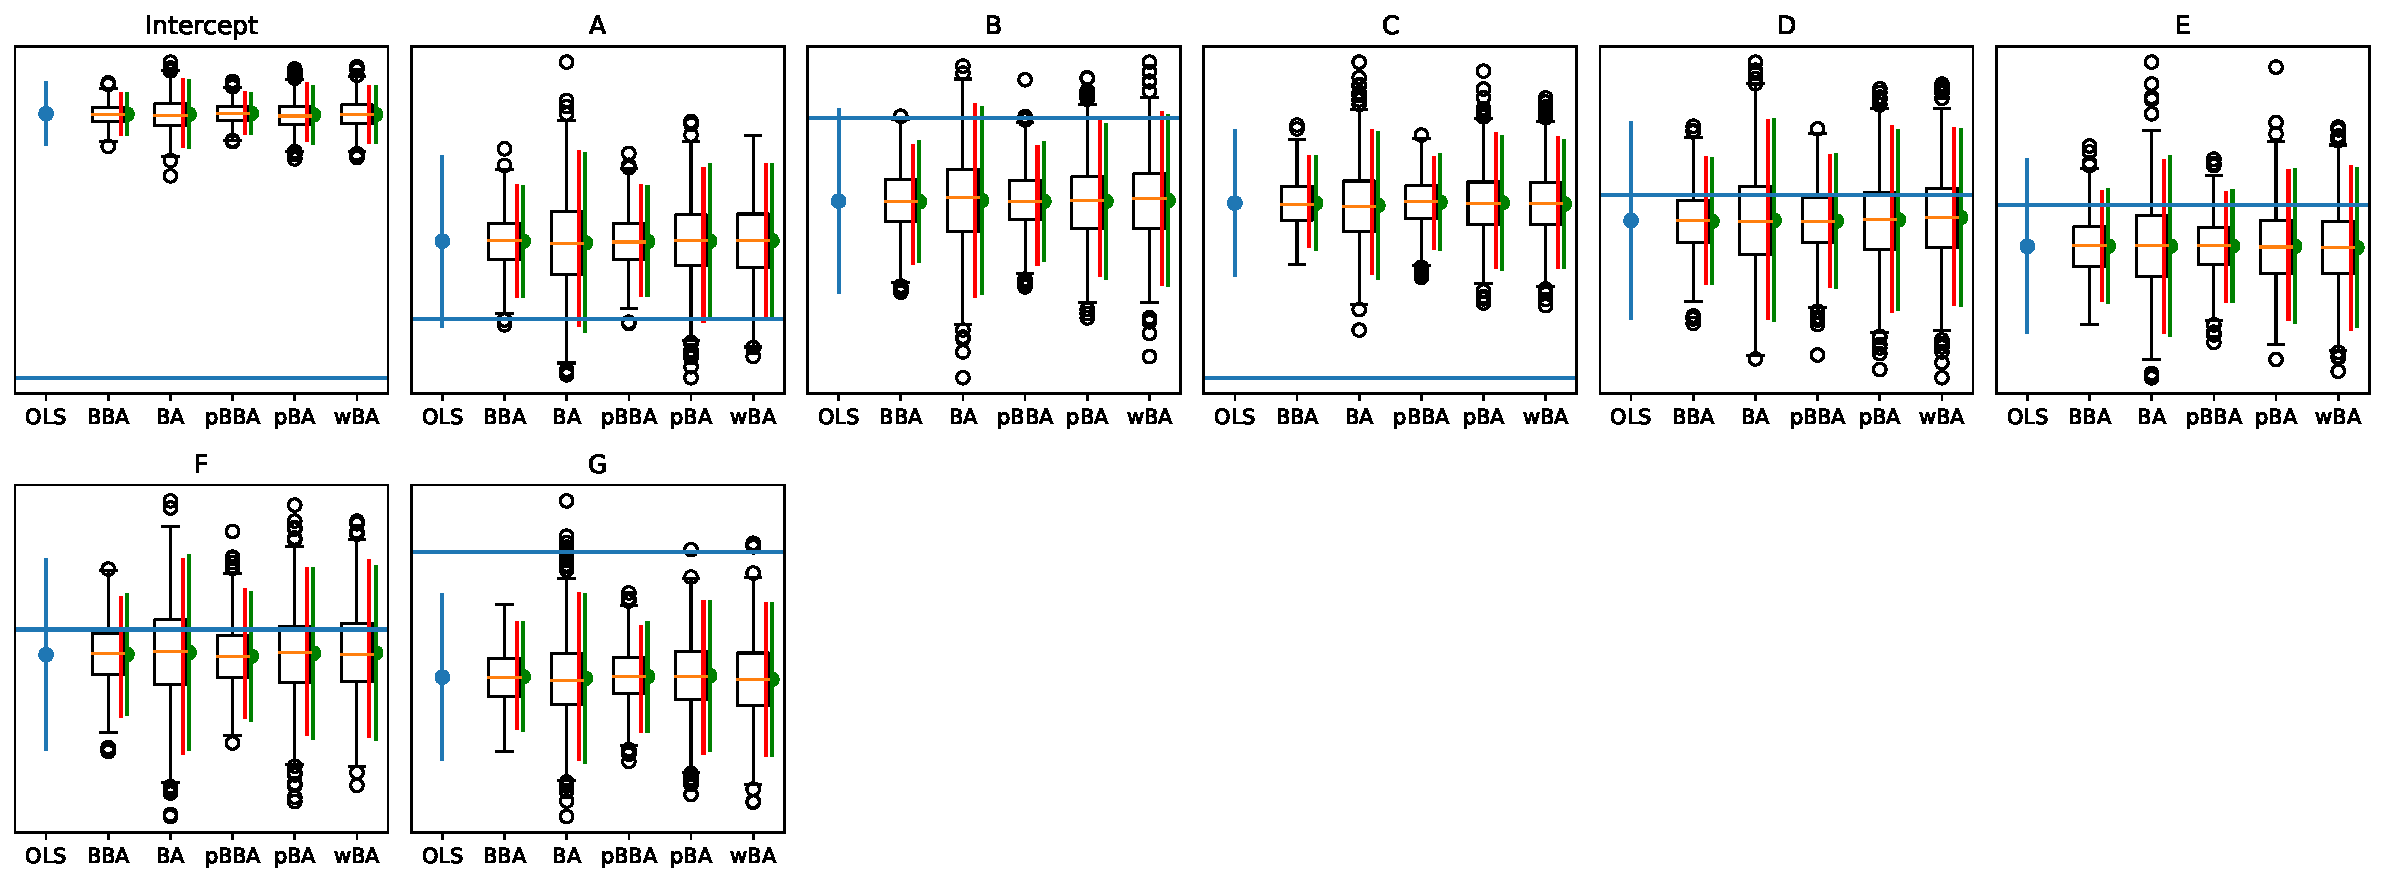
\includegraphics[width=\linewidth]{figures/wavesoldering-main-dist.pdf}
    \caption{Distribution of main effect coefficient estimates for the wave soldering dataset. 
        Blue: ols estimate $\pm$ std.dev. 
        For each bootstrap approach, boxplot: distribution, red: interquartile range, green: mean $\pm$ std.dev.}
    \label{fig:wavesoldering-main-dist}
% \end{figure}
% \begin{figure}
    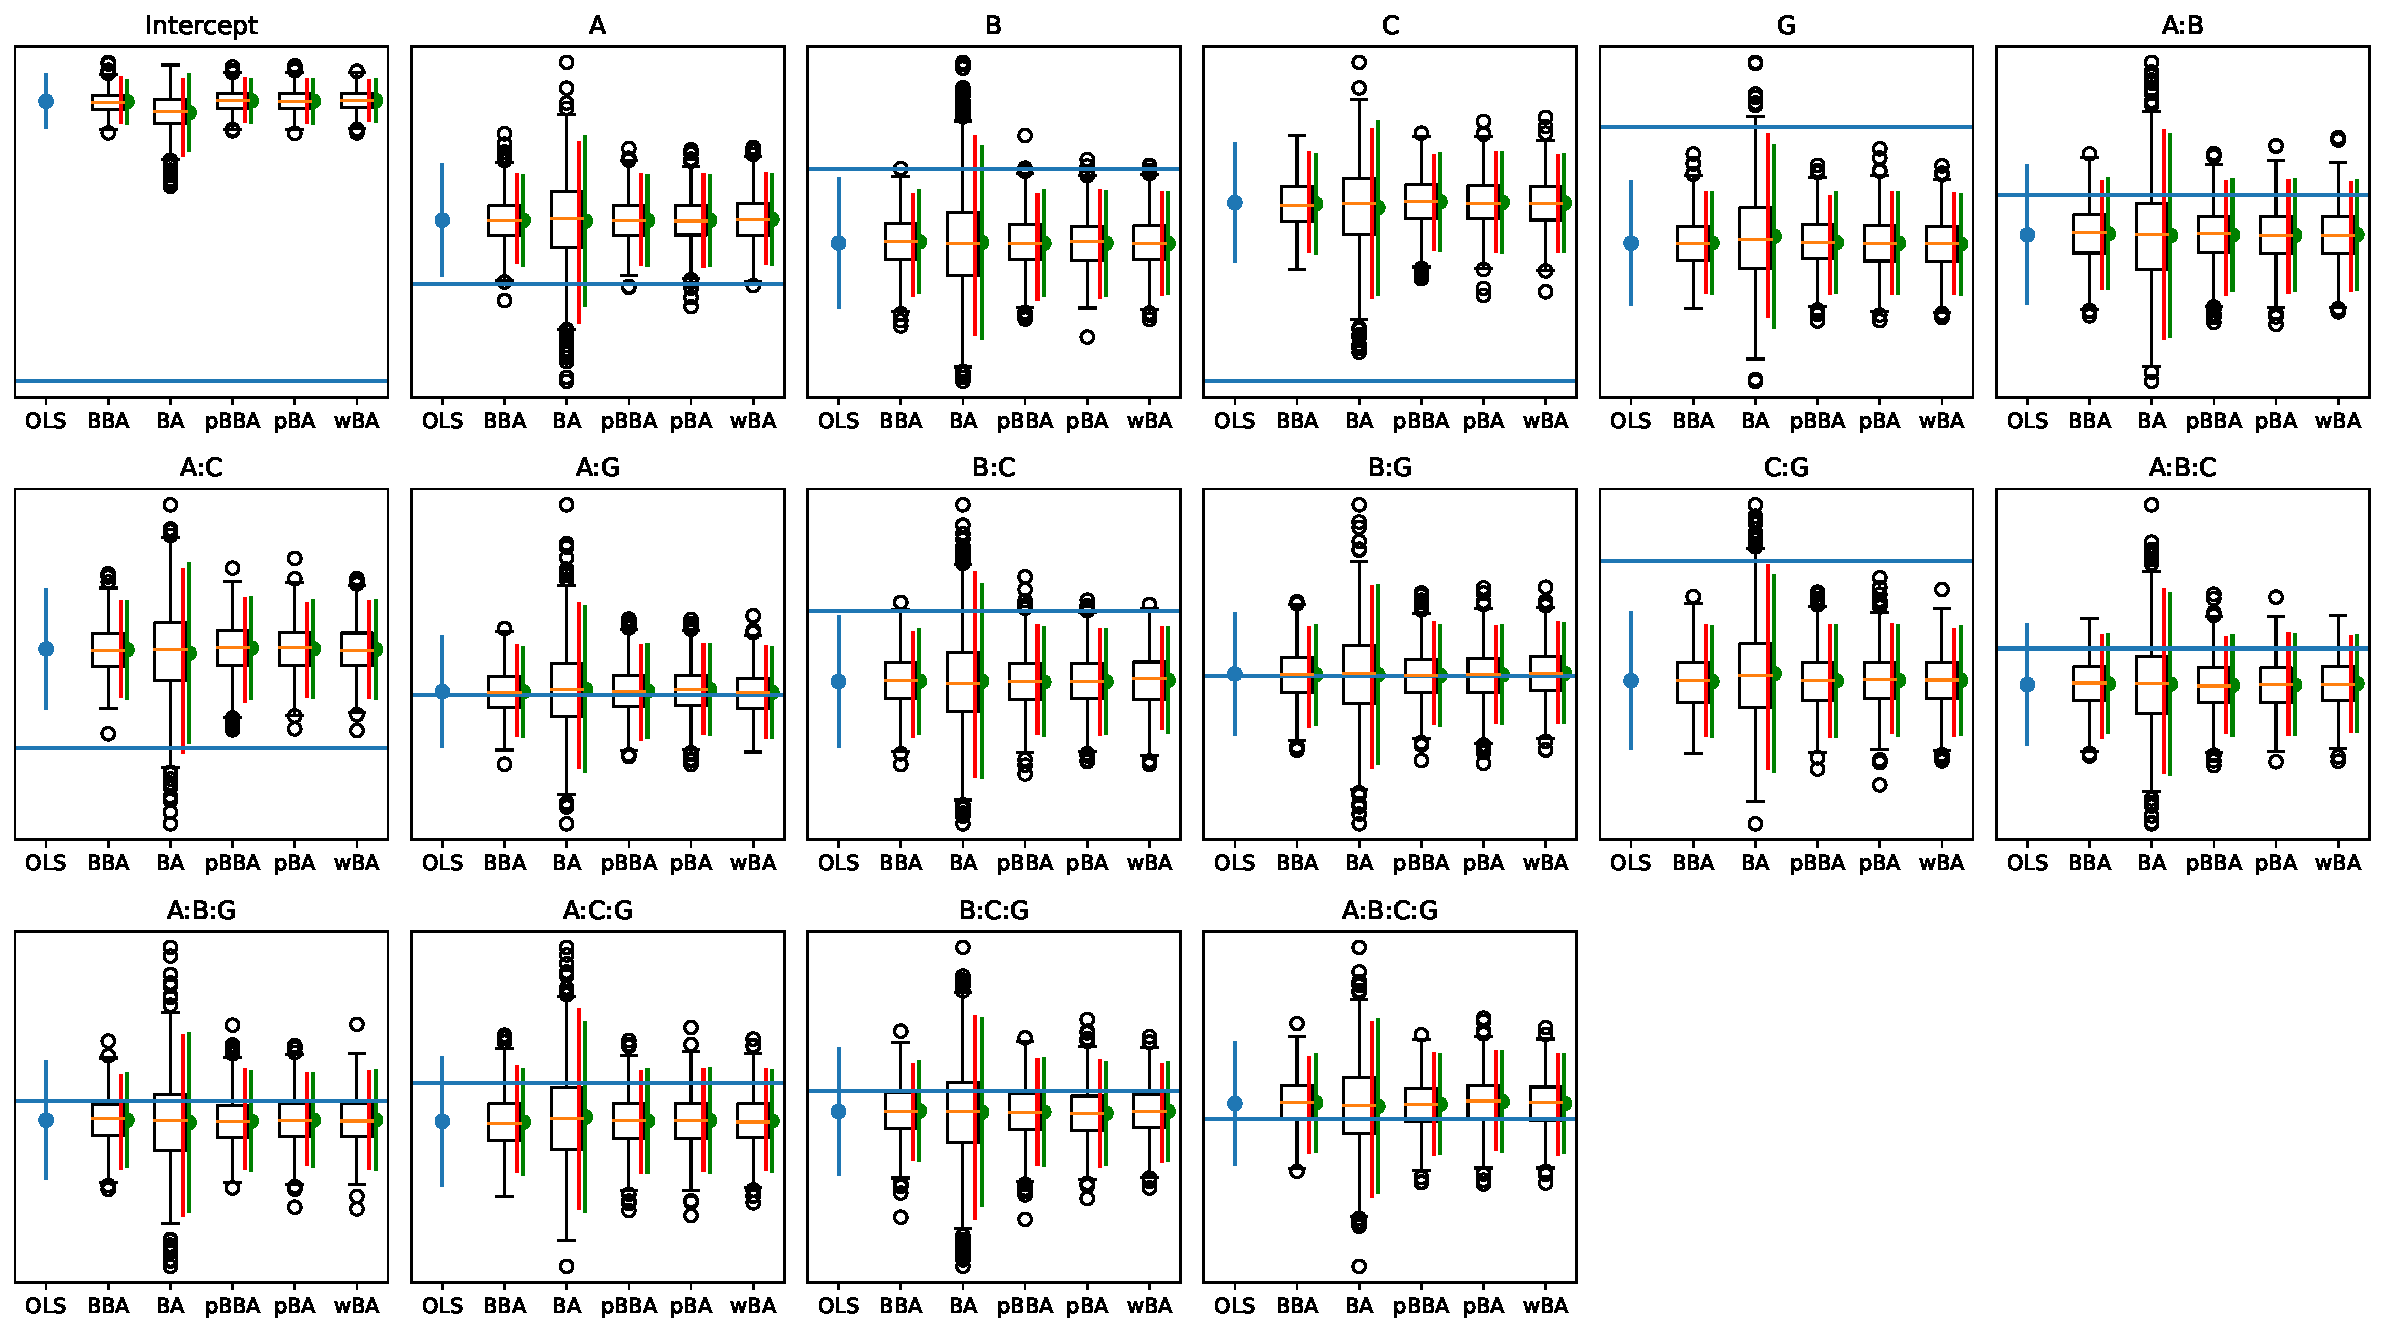
\includegraphics[width=\linewidth]{figures/wavesoldering-int-dist.pdf}
    \caption{Distribution of main effects and interaction coefficient estimates for the wave soldering dataset. 
        Blue: ols estimate $\pm$ std.dev. 
        For each bootstrap approach, boxplot: distribution, red: interquartile range, green: mean $\pm$ std.dev.}
    \label{fig:wavesoldering-main-int}
\end{figure}
\subsection{Main effects}
\begin{itemize}
    \item Formula: $Data \sim A + B + C + D + E + F + G$
    \item Number of bootstrap samples: 100
    \item Distribution of bootstrap sampled coefficients: Figure~\ref{fig:wavesoldering-main-dist}
\end{itemize}

\subsection{Interactions}
\begin{itemize}
    \item Formula: $Data \sim A + B + C + G + A:B + A:C + A:G + B:C + B:G + C:G + A:B:C + A:B:G + A:C:G + B:C:G + A:B:C:G$
    \item Number of bootstrap samples: 100
    \item Distribution of bootstrap sampled coefficients: Figure~\ref{fig:wavesoldering-main-int}
\end{itemize}

\subsection{Comparisons}
\begin{table}
\centering
\caption{BBA std. deviation of the regression coefficients for the wave soldering data.}
\label{tbl:wavesoldering-BBA}
\begin{tabular}{lrrrrrrrrrrrrrrrrrr}
\toprule
 & \multicolumn{3}{c}{Main} & \multicolumn{3}{c}{Interaction} \\
 & Regr. & Bootstrap & Delta & Regr. & Bootstrap & Delta \\
\midrule
Intercept & \red{0.299} & \red{0.194} & \red{-34.9} & \red{0.239} & \red{0.195} & \red{-18.2} \\
A & \red{0.299} & \red{0.193} & \red{-35.3} & \red{0.239} & \red{0.193} & \red{-19.3} \\
B & \red{0.299} & \red{0.196} & \red{-34.3} & \red{0.239} & \red{0.187} & \red{-21.5} \\
C & \red{0.299} & \red{0.191} & \red{-35.9} & \red{0.239} & \red{0.198} & \red{-17.0} \\
D & 0.299 & 0.190 & -36.4 &  &  &  \\
E & 0.299 & 0.195 & -34.8 &  &  &  \\
F & 0.299 & 0.188 & -37.0 &  &  &  \\
G & \red{0.299} & \red{0.194} & \red{-35.1} & \red{0.239} & \red{0.196} & \red{-17.9} \\
A:B &  &  &  & 0.239 & 0.190 & -20.4 \\
A:C &  &  &  & \red{0.239} & \red{0.194} & \red{-18.8} \\
A:G &  &  &  & 0.239 & 0.193 & -18.9 \\
B:C &  &  &  & \red{0.239} & \red{0.190} & \red{-20.4} \\
B:G &  &  &  & 0.239 & 0.194 & -18.7 \\
C:G &  &  &  & \red{0.239} & \red{0.195} & \red{-18.4} \\
A:B:C &  &  &  & 0.239 & 0.194 & -18.6 \\
A:B:G &  &  &  & 0.239 & 0.190 & -20.2 \\
A:C:G &  &  &  & 0.239 & 0.195 & -18.2 \\
B:C:G &  &  &  & 0.239 & 0.188 & -21.1 \\
A:B:C:G &  &  &  & 0.239 & 0.190 & -20.5 \\
\bottomrule
\end{tabular}
\end{table}

\begin{table}
\centering
\caption{BA std. deviation of the regression coefficients for the wave soldering data.}
\label{tbl:wavesoldering-BA}
\begin{tabular}{lrrrrrrrrrrrrrrrrrr}
\toprule
 & \multicolumn{3}{c}{Main} & \multicolumn{3}{c}{Interaction} \\
 & Regr. & Bootstrap & Delta & Regr. & Bootstrap & Delta \\
\midrule
Intercept & \red{0.299} & \red{0.320} & \red{7.1} & \red{0.239} & \red{0.346} & \red{45.2} \\
A & \red{0.299} & \red{0.313} & \red{4.8} & \red{0.239} & \red{0.366} & \red{53.2} \\
B & \red{0.299} & \red{0.306} & \red{2.3} & \red{0.239} & \red{0.355} & \red{48.9} \\
C & \red{0.299} & \red{0.301} & \red{0.7} & \red{0.239} & \red{0.349} & \red{46.2} \\
D & 0.299 & 0.306 & 2.4 &  &  &  \\
E & 0.299 & 0.310 & 3.7 &  &  &  \\
F & 0.299 & 0.307 & 2.7 &  &  &  \\
G & \red{0.299} & \red{0.302} & \red{1.2} & \red{0.239} & \red{0.357} & \red{49.5} \\
A:B &  &  &  & 0.239 & 0.351 & 46.9 \\
A:C &  &  &  & \red{0.239} & \red{0.361} & \red{51.4} \\
A:G &  &  &  & 0.239 & 0.358 & 50.1 \\
B:C &  &  &  & \red{0.239} & \red{0.354} & \red{48.6} \\
B:G &  &  &  & 0.239 & 0.352 & 47.4 \\
C:G &  &  &  & \red{0.239} & \red{0.345} & \red{44.7} \\
A:B:C &  &  &  & 0.239 & 0.358 & 50.1 \\
A:B:G &  &  &  & 0.239 & 0.363 & 52.2 \\
A:C:G &  &  &  & 0.239 & 0.354 & 48.2 \\
B:C:G &  &  &  & 0.239 & 0.354 & 48.5 \\
A:B:C:G &  &  &  & 0.239 & 0.339 & 42.3 \\
\bottomrule
\end{tabular}
\end{table}

\begin{table}
\centering
\caption{pBBA std. deviation of the regression coefficients for the wave soldering data.}
\label{tbl:wavesoldering-pBBA}
\begin{tabular}{lrrrrrrrrrrrrrrrrrr}
\toprule
 & \multicolumn{3}{c}{Main} & \multicolumn{3}{c}{Interaction} \\
 & Regr. & Bootstrap & Delta & Regr. & Bootstrap & Delta \\
\midrule
Intercept & \red{0.299} & \red{0.192} & \red{-35.6} & \red{0.239} & \red{0.192} & \red{-19.4} \\
A & \red{0.299} & \red{0.191} & \red{-35.9} & \red{0.239} & \red{0.191} & \red{-19.8} \\
B & \red{0.299} & \red{0.194} & \red{-35.2} & \red{0.239} & \red{0.194} & \red{-18.9} \\
C & \red{0.299} & \red{0.194} & \red{-35.0} & \red{0.239} & \red{0.194} & \red{-18.6} \\
D & 0.299 & 0.201 & -32.8 &  &  &  \\
E & 0.299 & 0.191 & -36.0 &  &  &  \\
F & 0.299 & 0.201 & -32.6 &  &  &  \\
G & \red{0.299} & \red{0.196} & \red{-34.4} & \red{0.239} & \red{0.196} & \red{-17.8} \\
A:B &  &  &  & 0.239 & 0.191 & -19.8 \\
A:C &  &  &  & \red{0.239} & \red{0.203} & \red{-14.9} \\
A:G &  &  &  & 0.239 & 0.201 & -15.7 \\
B:C &  &  &  & \red{0.239} & \red{0.198} & \red{-17.0} \\
B:G &  &  &  & 0.239 & 0.198 & -17.0 \\
C:G &  &  &  & \red{0.239} & \red{0.195} & \red{-18.2} \\
A:B:C &  &  &  & 0.239 & 0.196 & -17.7 \\
A:B:G &  &  &  & 0.239 & 0.201 & -15.7 \\
A:C:G &  &  &  & 0.239 & 0.191 & -19.9 \\
B:C:G &  &  &  & 0.239 & 0.201 & -15.9 \\
A:B:C:G &  &  &  & 0.239 & 0.194 & -18.7 \\
\bottomrule
\end{tabular}
\end{table}

\begin{table}
\centering
\caption{pBA std. deviation of the regression coefficients for the wave soldering data.}
\label{tbl:wavesoldering-pBA}
\begin{tabular}{lrrrrrrrrrrrrrrrrrr}
\toprule
 & \multicolumn{3}{c}{Main} & \multicolumn{3}{c}{Interaction} \\
 & Regr. & Bootstrap & Delta & Regr. & Bootstrap & Delta \\
\midrule
Intercept & \red{0.299} & \red{0.273} & \red{-8.7} & \red{0.239} & \red{0.198} & \red{-17.0} \\
A & \red{0.299} & \red{0.268} & \red{-10.2} & \red{0.239} & \red{0.193} & \red{-19.0} \\
B & \red{0.299} & \red{0.252} & \red{-15.6} & \red{0.239} & \red{0.191} & \red{-20.0} \\
C & \red{0.299} & \red{0.274} & \red{-8.2} & \red{0.239} & \red{0.200} & \red{-16.2} \\
D & 0.299 & 0.273 & -8.7 &  &  &  \\
E & 0.299 & 0.264 & -11.6 &  &  &  \\
F & 0.299 & 0.268 & -10.3 &  &  &  \\
G & \red{0.299} & \red{0.269} & \red{-10.1} & \red{0.239} & \red{0.196} & \red{-17.9} \\
A:B &  &  &  & 0.239 & 0.191 & -19.8 \\
A:C &  &  &  & \red{0.239} & \red{0.194} & \red{-18.8} \\
A:G &  &  &  & 0.239 & 0.195 & -18.1 \\
B:C &  &  &  & \red{0.239} & \red{0.190} & \red{-20.3} \\
B:G &  &  &  & 0.239 & 0.193 & -19.2 \\
C:G &  &  &  & \red{0.239} & \red{0.193} & \red{-19.2} \\
A:B:C &  &  &  & 0.239 & 0.198 & -17.2 \\
A:B:G &  &  &  & 0.239 & 0.188 & -21.3 \\
A:C:G &  &  &  & 0.239 & 0.193 & -19.3 \\
B:C:G &  &  &  & 0.239 & 0.193 & -19.0 \\
A:B:C:G &  &  &  & 0.239 & 0.194 & -18.5 \\
\bottomrule
\end{tabular}
\end{table}

\begin{table}
\centering
\caption{wBA std. deviation of the regression coefficients for the wave soldering data.}
\label{tbl:wavesoldering-wBA}
\begin{tabular}{lrrrrrrrrrrrrrrrrrr}
\toprule
 & \multicolumn{3}{c}{Main} & \multicolumn{3}{c}{Interaction} \\
 & Regr. & Bootstrap & Delta & Regr. & Bootstrap & Delta \\
\midrule
Intercept & \red{0.299} & \red{0.268} & \red{-10.1} & \red{0.239} & \red{0.186} & \red{-22.2} \\
A & \red{0.299} & \red{0.268} & \red{-10.4} & \red{0.239} & \red{0.193} & \red{-19.0} \\
B & \red{0.299} & \red{0.277} & \red{-7.3} & \red{0.239} & \red{0.186} & \red{-22.2} \\
C & \red{0.299} & \red{0.261} & \red{-12.5} & \red{0.239} & \red{0.195} & \red{-18.1} \\
D & 0.299 & 0.269 & -10.0 &  &  &  \\
E & 0.299 & 0.274 & -8.2 &  &  &  \\
F & 0.299 & 0.272 & -9.0 &  &  &  \\
G & \red{0.299} & \red{0.274} & \red{-8.3} & \red{0.239} & \red{0.195} & \red{-18.4} \\
A:B &  &  &  & 0.239 & 0.187 & -21.5 \\
A:C &  &  &  & \red{0.239} & \red{0.195} & \red{-18.4} \\
A:G &  &  &  & 0.239 & 0.195 & -18.4 \\
B:C &  &  &  & \red{0.239} & \red{0.192} & \red{-19.6} \\
B:G &  &  &  & 0.239 & 0.195 & -18.3 \\
C:G &  &  &  & \red{0.239} & \red{0.190} & \red{-20.5} \\
A:B:C &  &  &  & 0.239 & 0.189 & -20.7 \\
A:B:G &  &  &  & 0.239 & 0.200 & -16.1 \\
A:C:G &  &  &  & 0.239 & 0.188 & -21.1 \\
B:C:G &  &  &  & 0.239 & 0.185 & -22.5 \\
A:B:C:G &  &  &  & 0.239 & 0.190 & -20.4 \\
\bottomrule
\end{tabular}
\end{table}



\clearpage

\section{Piston simulator}
\begin{figure}
    \centering
    \begin{subfigure}{\textwidth}
        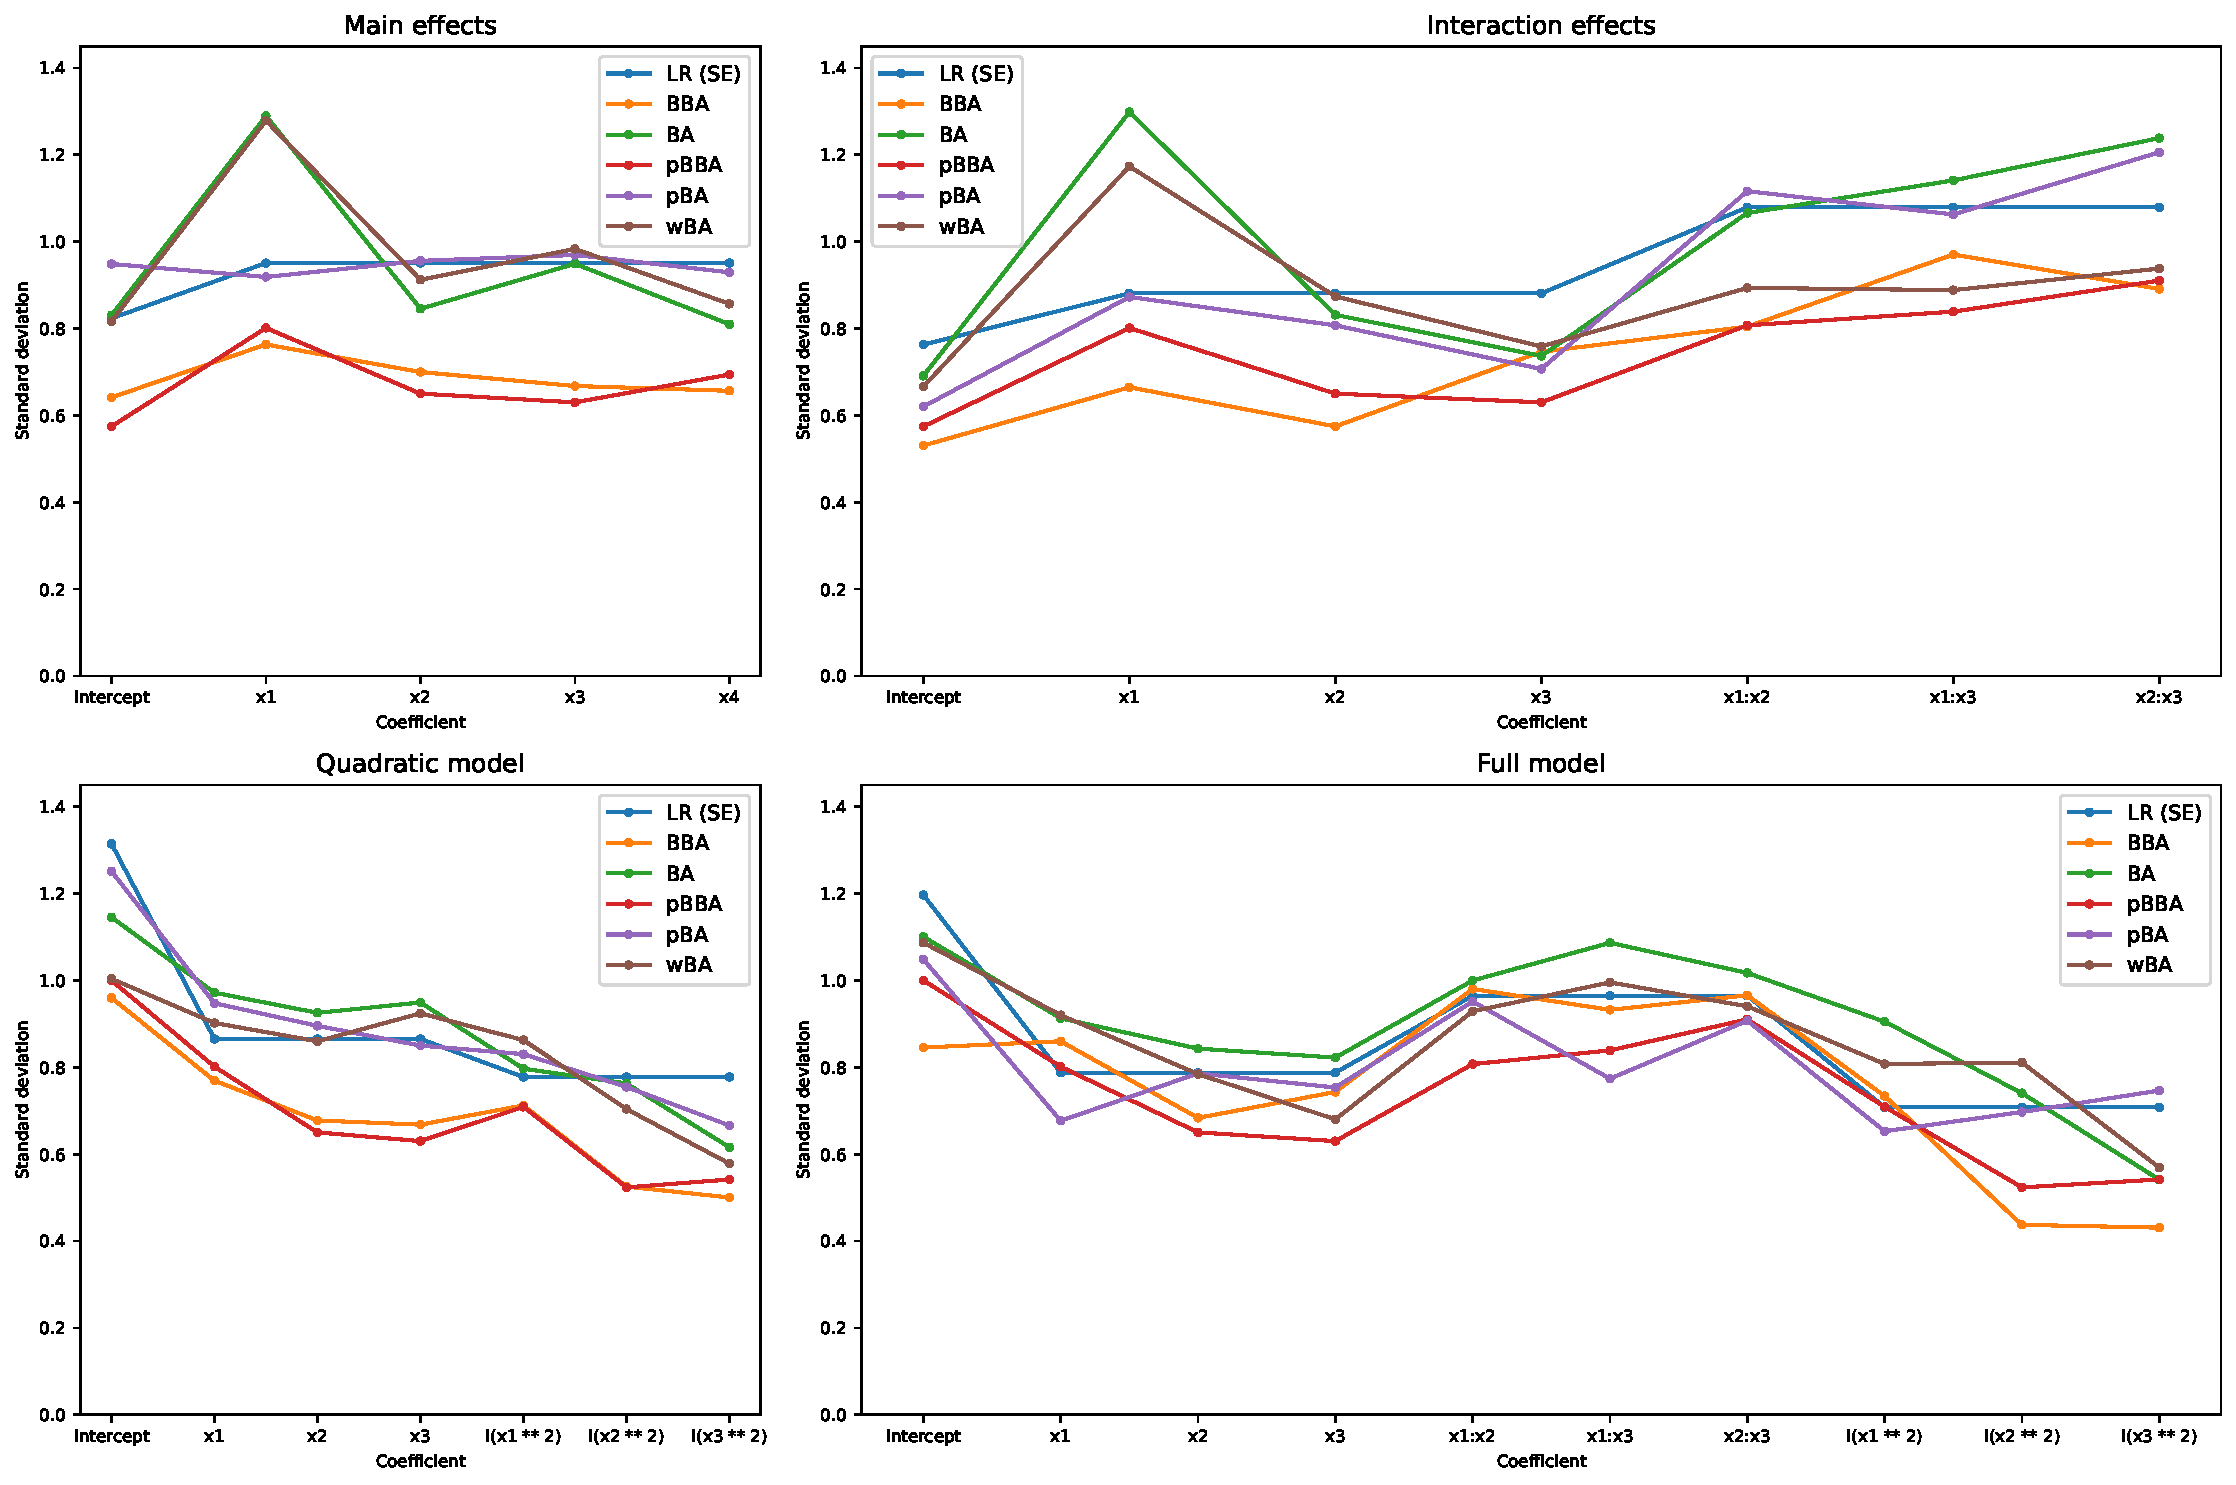
\includegraphics[width=0.8\linewidth]{figures/piston-std.pdf}
        \caption{100 bootstrap samples}
        \label{fig:piston-std-100}
    \end{subfigure}
    \begin{subfigure}{\textwidth}
        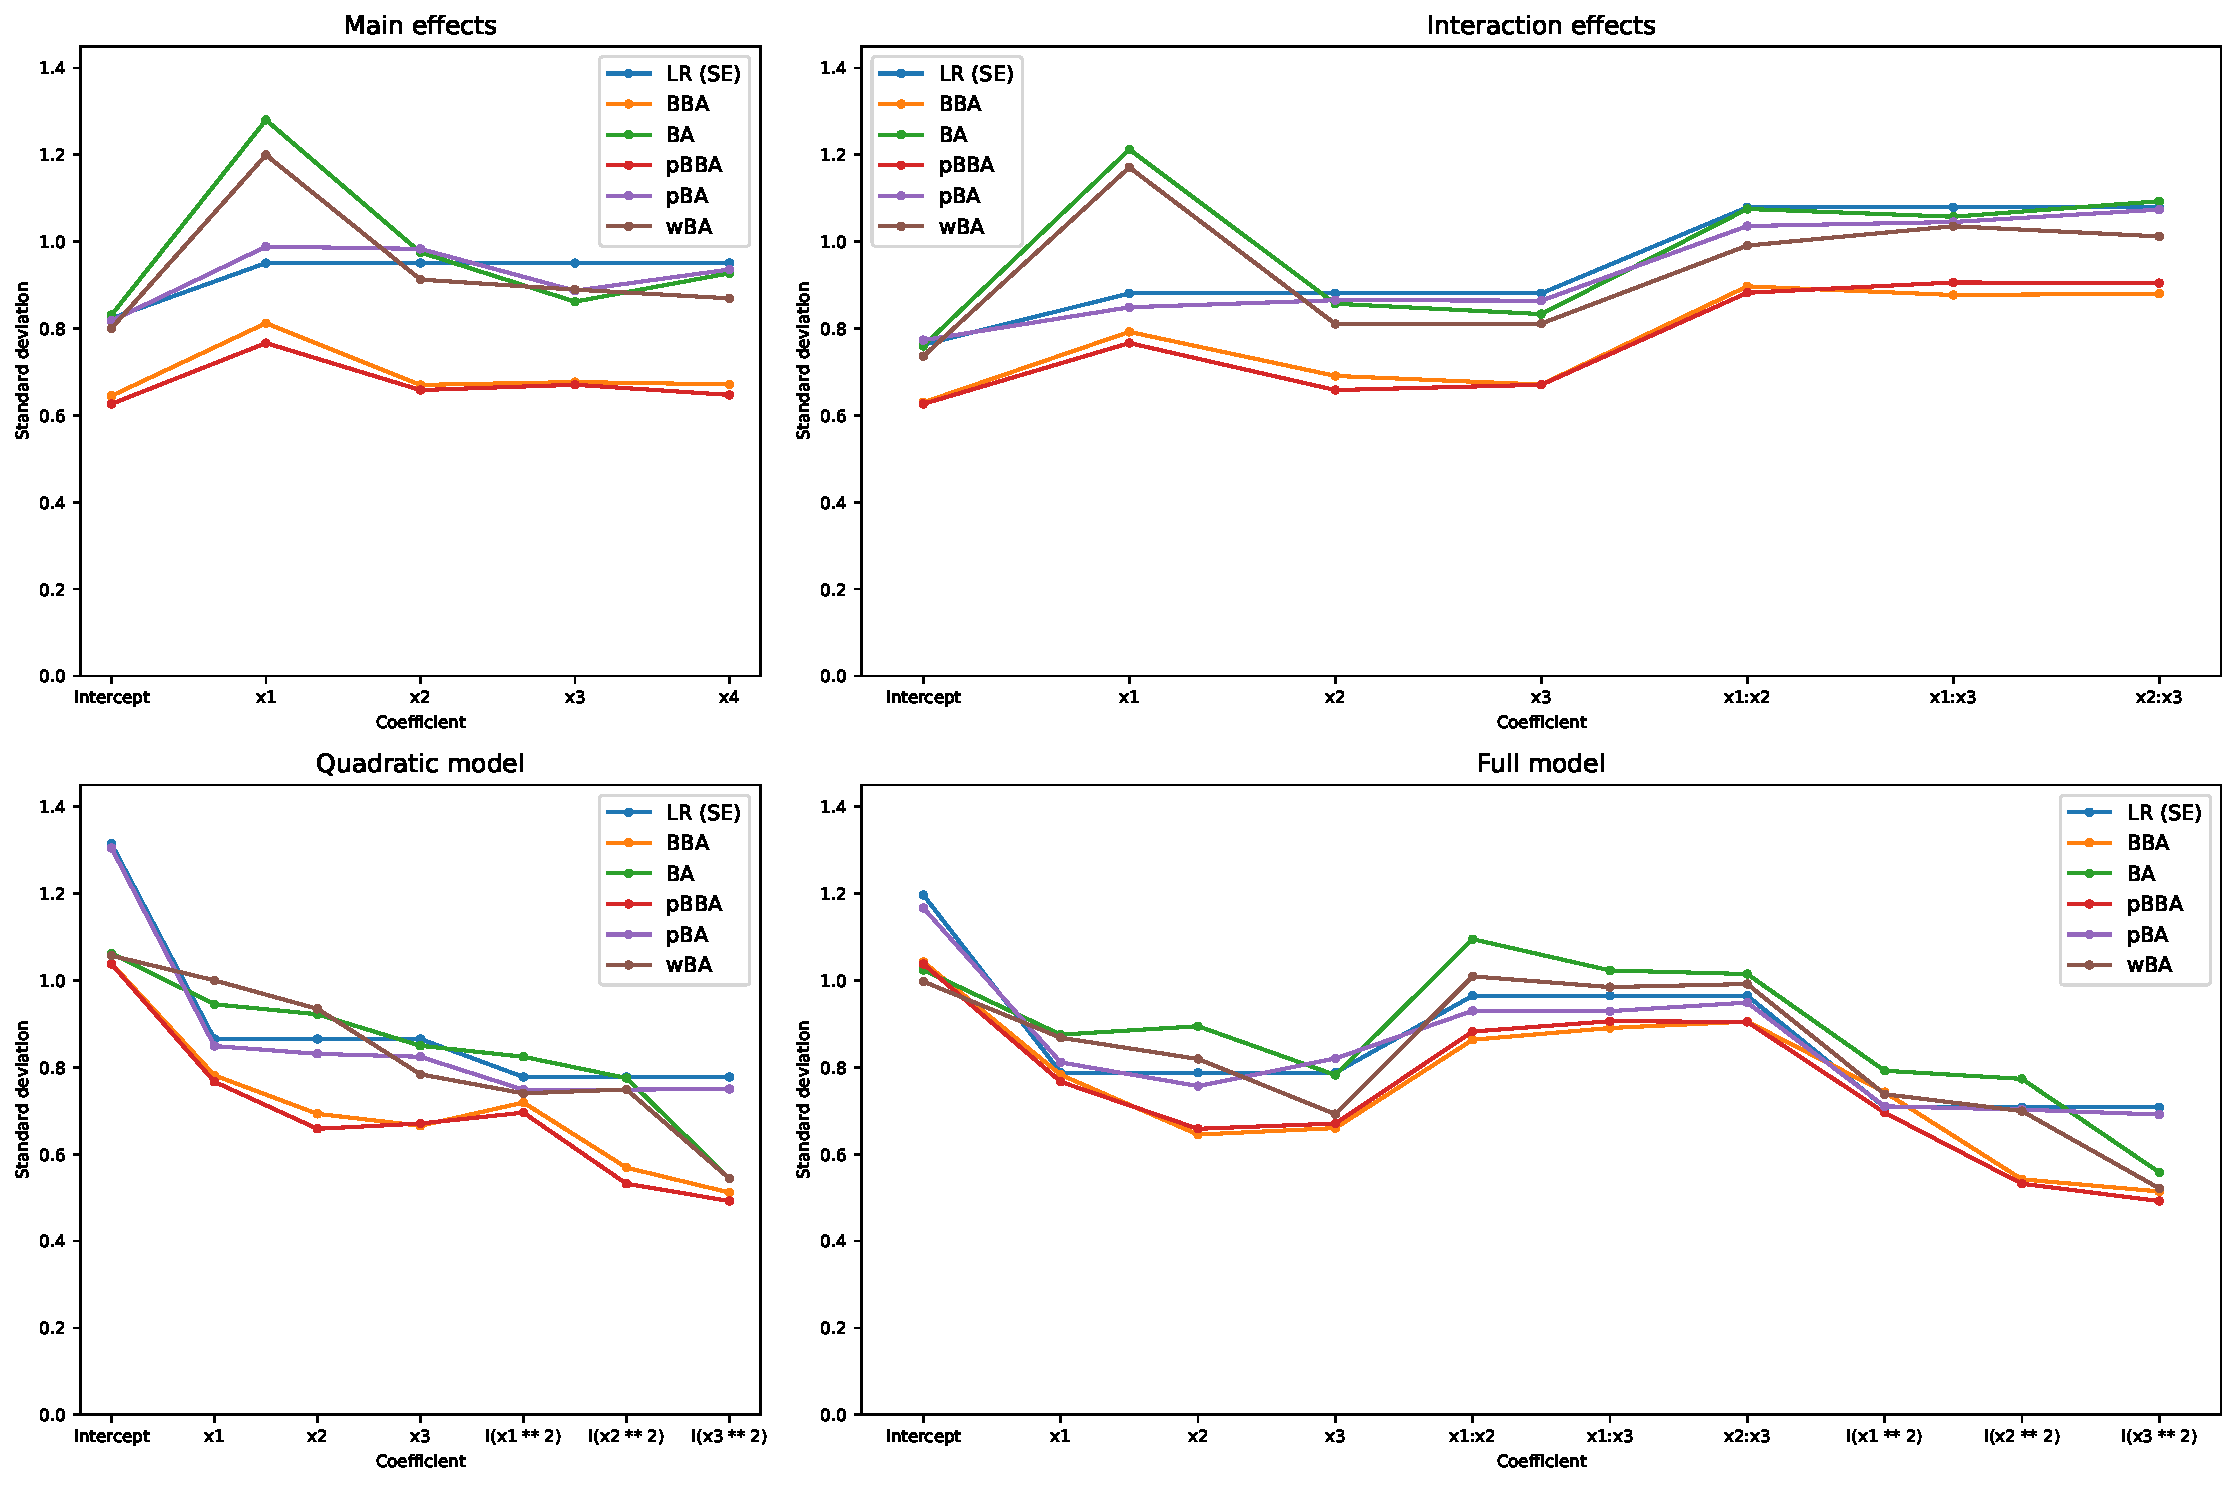
\includegraphics[width=0.8\linewidth]{figures/piston-std-500.pdf}
        \caption{500 bootstrap samples}
        \label{fig:piston-std-500}
    \end{subfigure}
    \begin{subfigure}{\textwidth}
        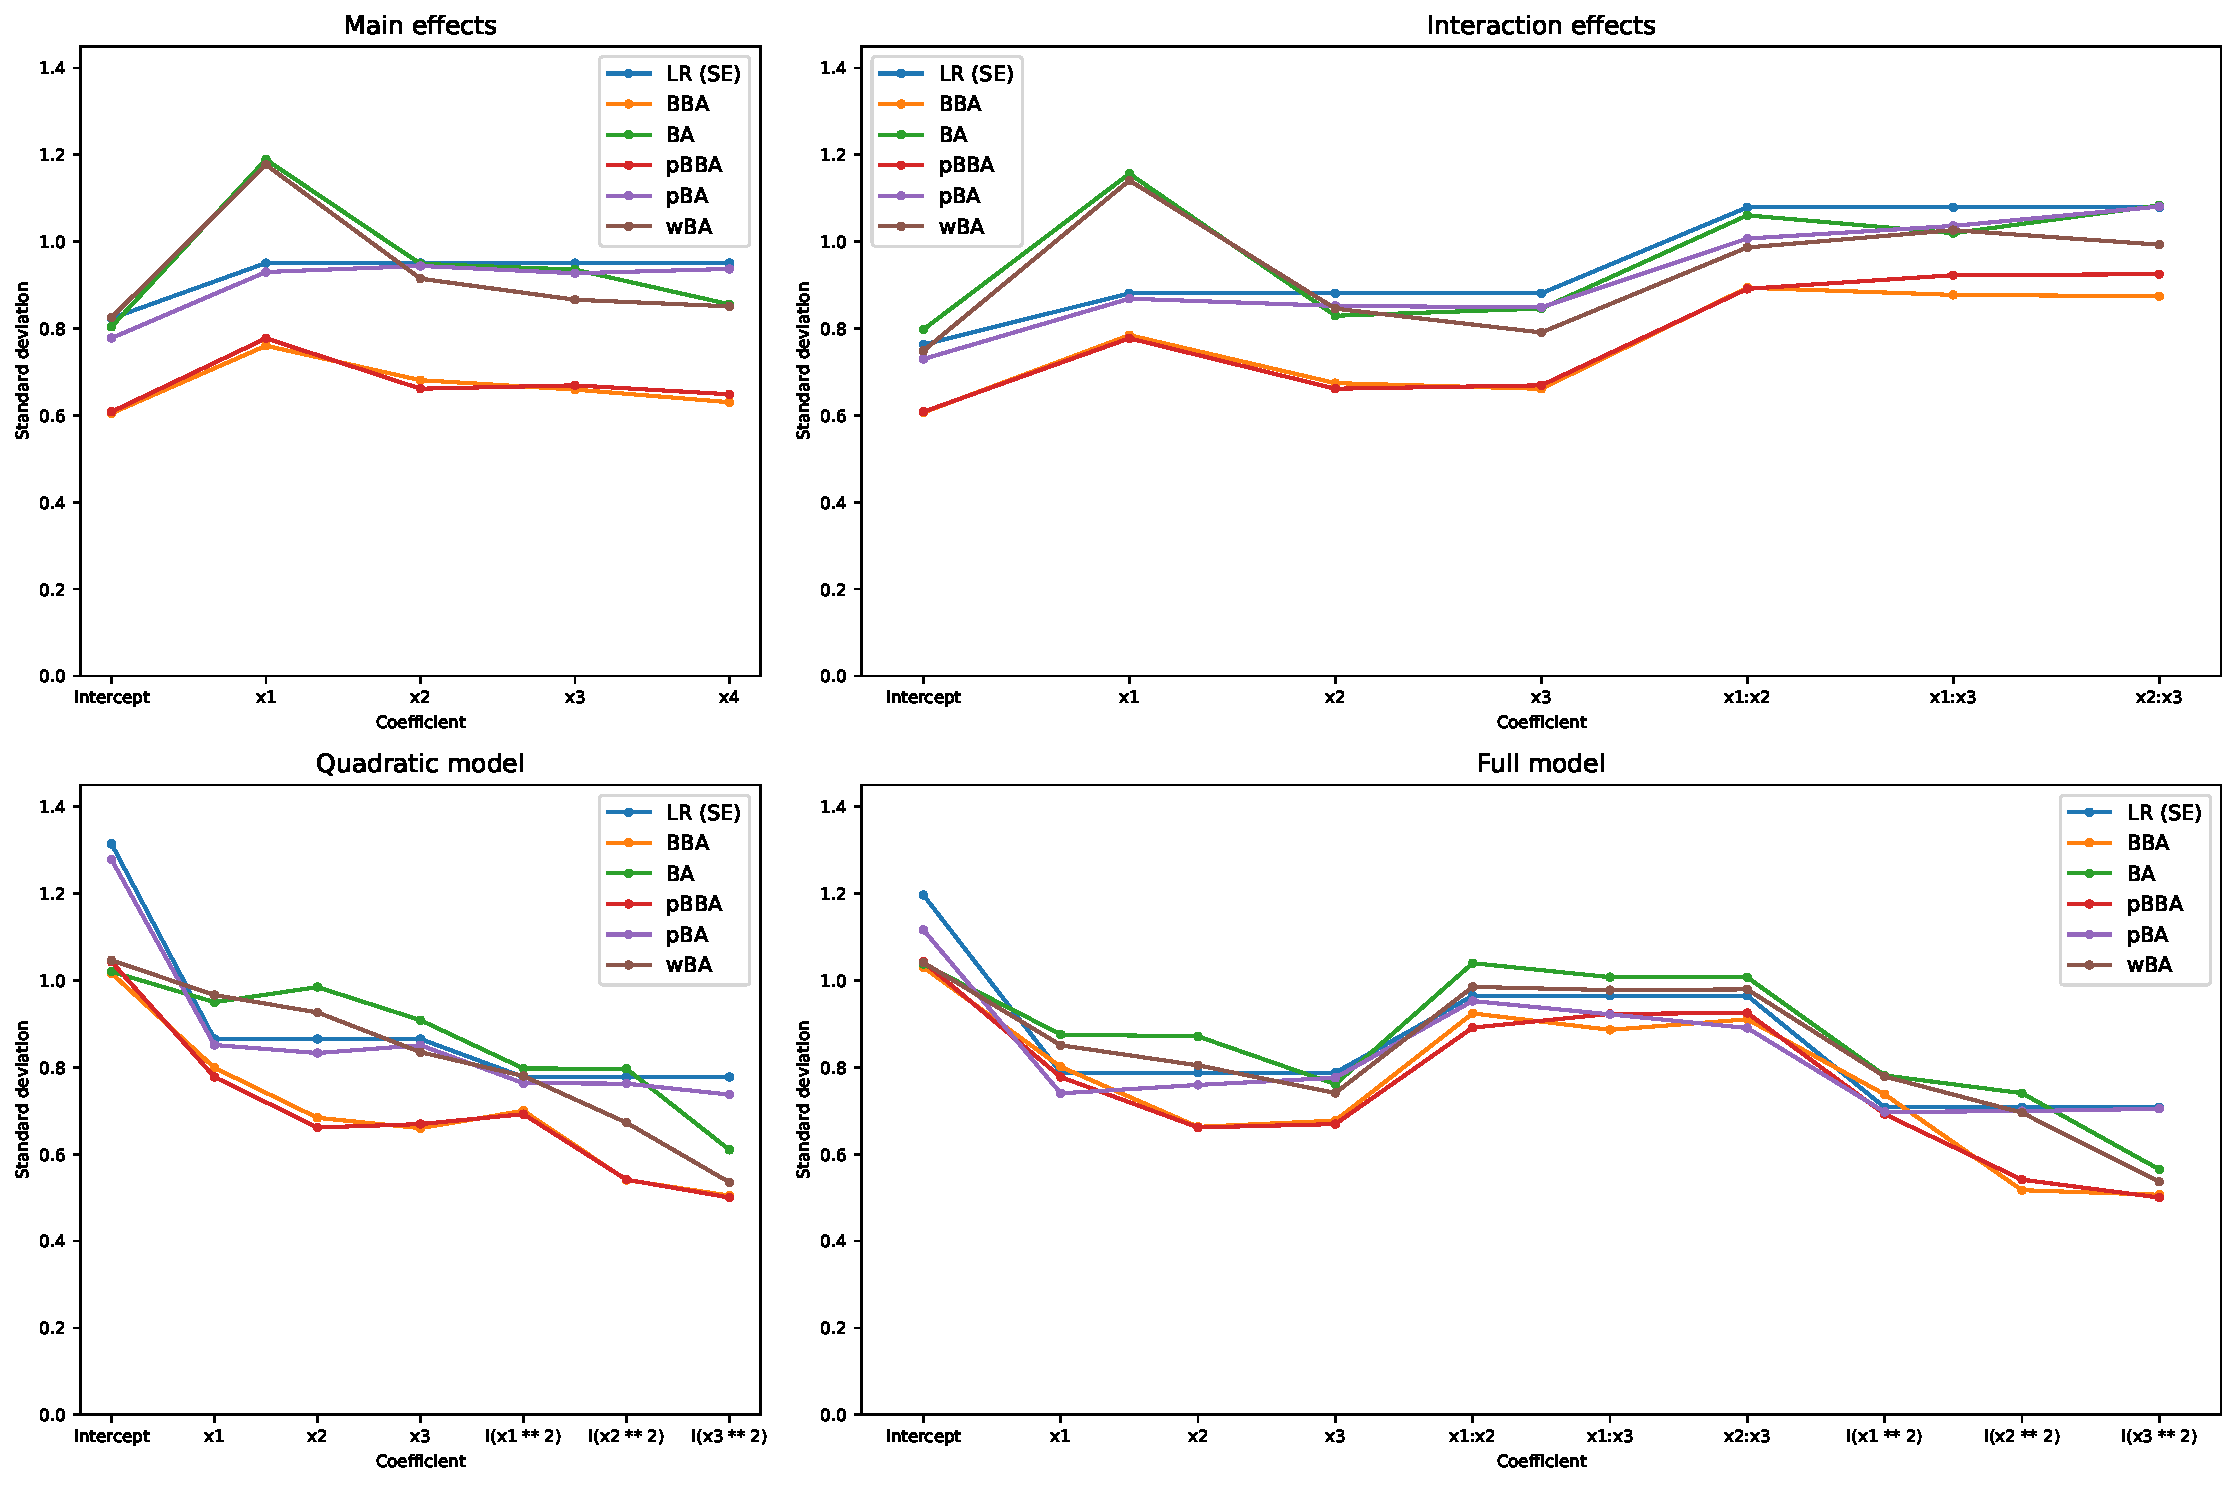
\includegraphics[width=0.8\linewidth]{figures/piston-std-1000.pdf}
        \caption{1000 bootstrap samples}
        \label{fig:piston-std-1000}
    \end{subfigure}
    \caption{Std.dev. of coefficients for piston simulator}
    \label{fig:piston-std}
\end{figure}

\begin{figure}
    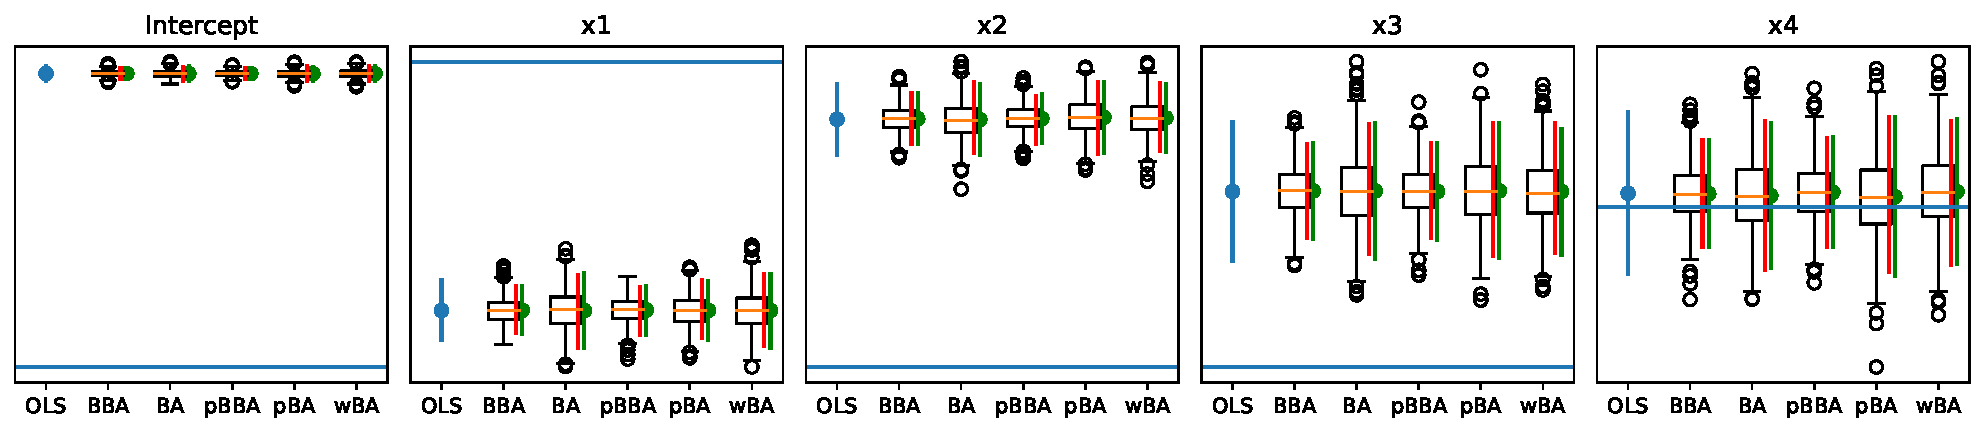
\includegraphics[width=\linewidth]{figures/piston-main-dist.pdf}
    \caption{Distribution of main effect coefficient estimates for the piston simulation. 
        Blue: ols estimate $\pm$ std.dev. 
        For each bootstrap approach, boxplot: distribution, red: interquartile range, green: mean $\pm$ std.dev.}
    \label{fig:piston-main-dist}
% \end{figure}
% \begin{figure}
    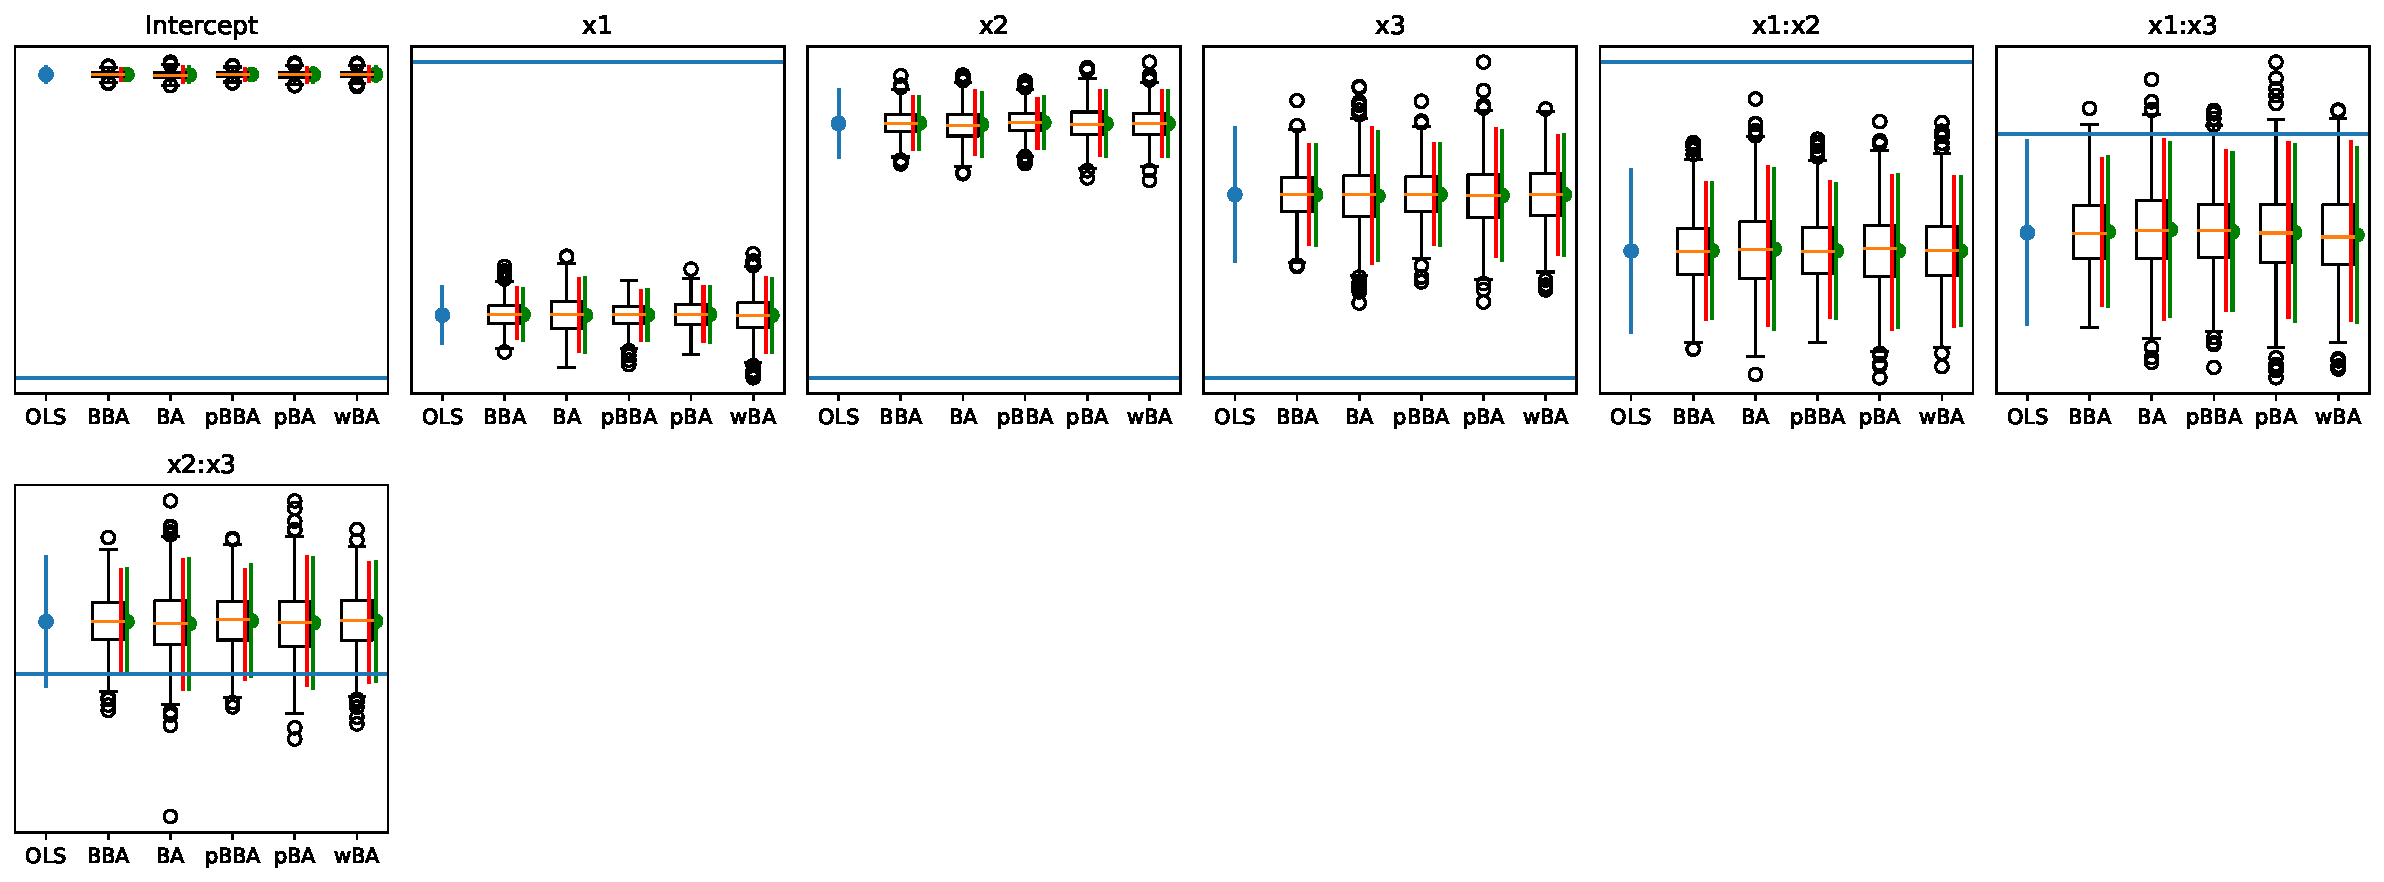
\includegraphics[width=\linewidth]{figures/piston-int-dist.pdf}
    \caption{Distribution of main effects and interaction coefficient estimates for the piston simulation. 
        Blue: ols estimate $\pm$ std.dev. 
        For each bootstrap approach, boxplot: distribution, red: interquartile range, green: mean $\pm$ std.dev.}
    \label{fig:piston-int-dist}
    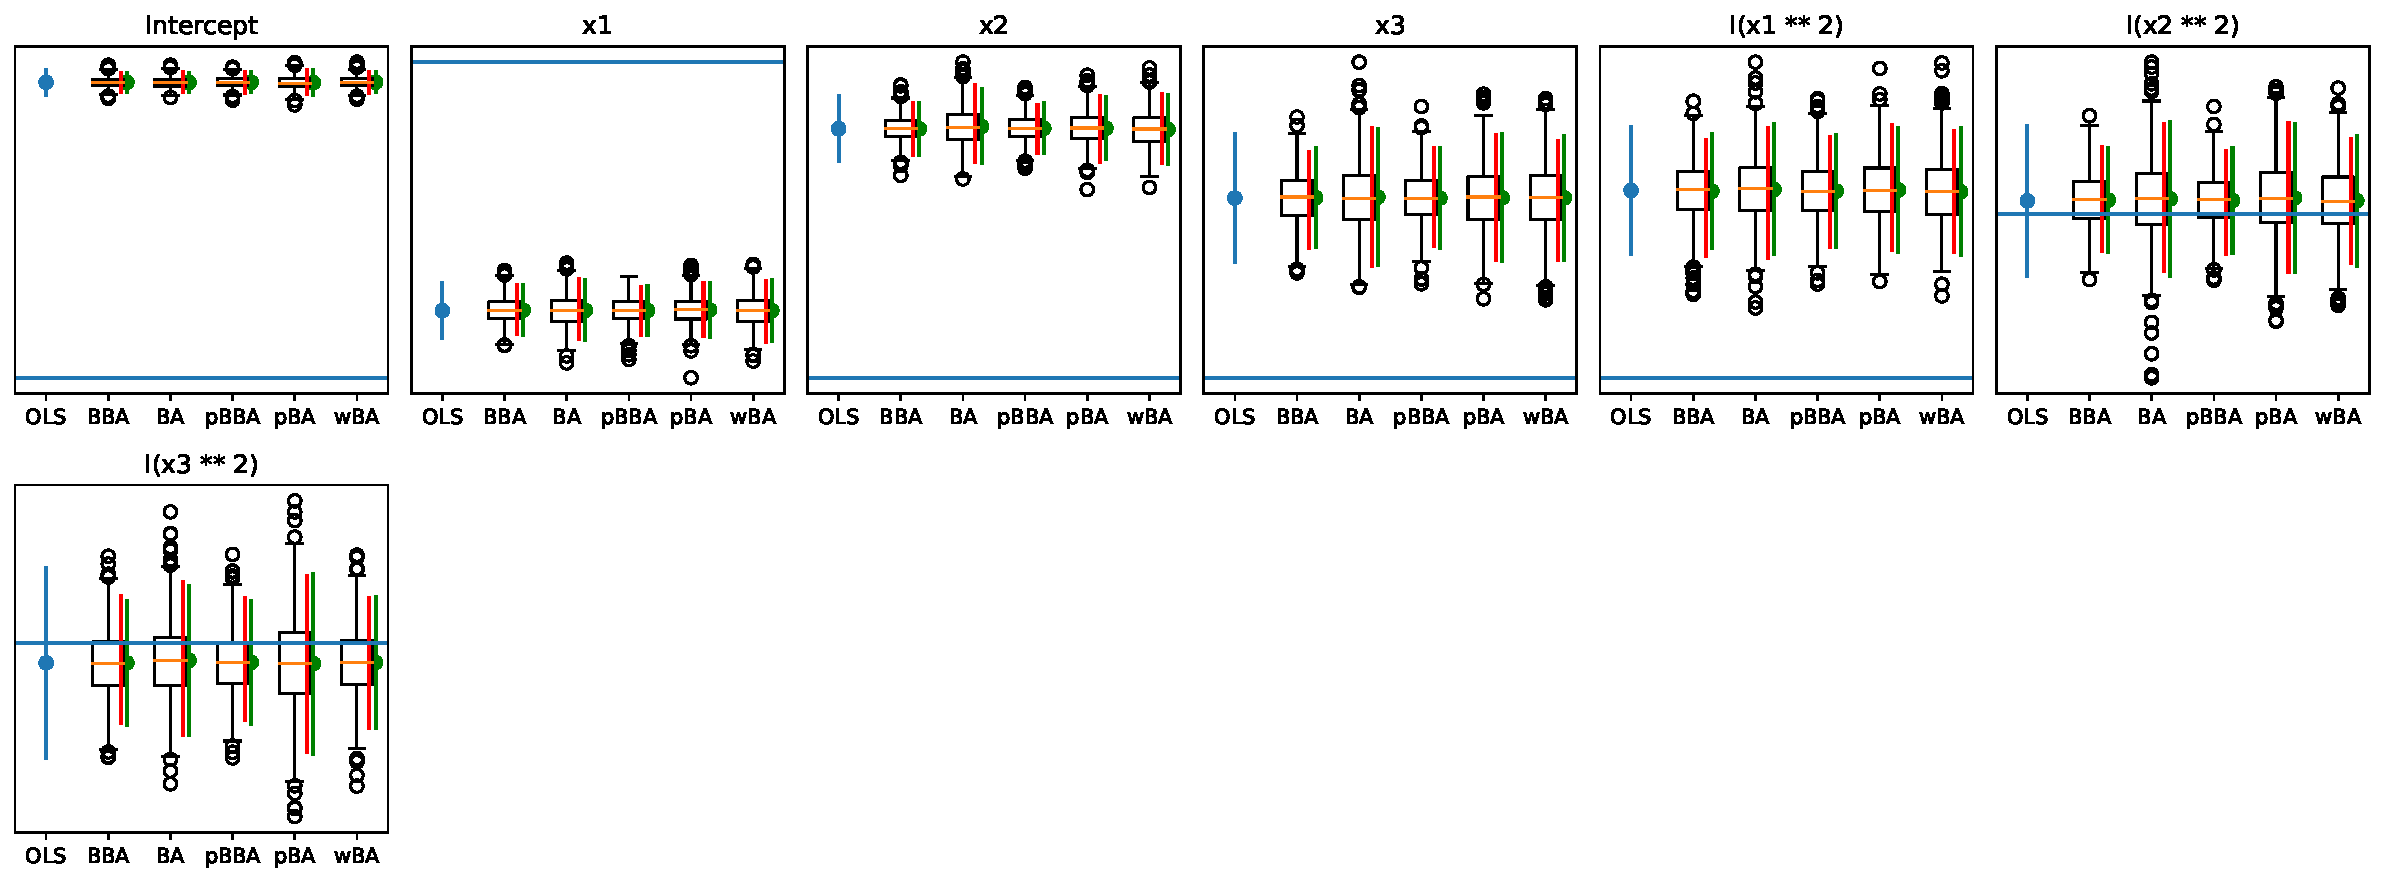
\includegraphics[width=\linewidth]{figures/piston-quadratic-dist.pdf}
    \caption{Distribution of main effects and quadratic coefficient estimates for the piston simulation. 
        Blue: ols estimate $\pm$ std.dev. 
        For each bootstrap approach, boxplot: distribution, red: interquartile range, green: mean $\pm$ std.dev.}
    \label{fig:piston-quadratic-dist}
    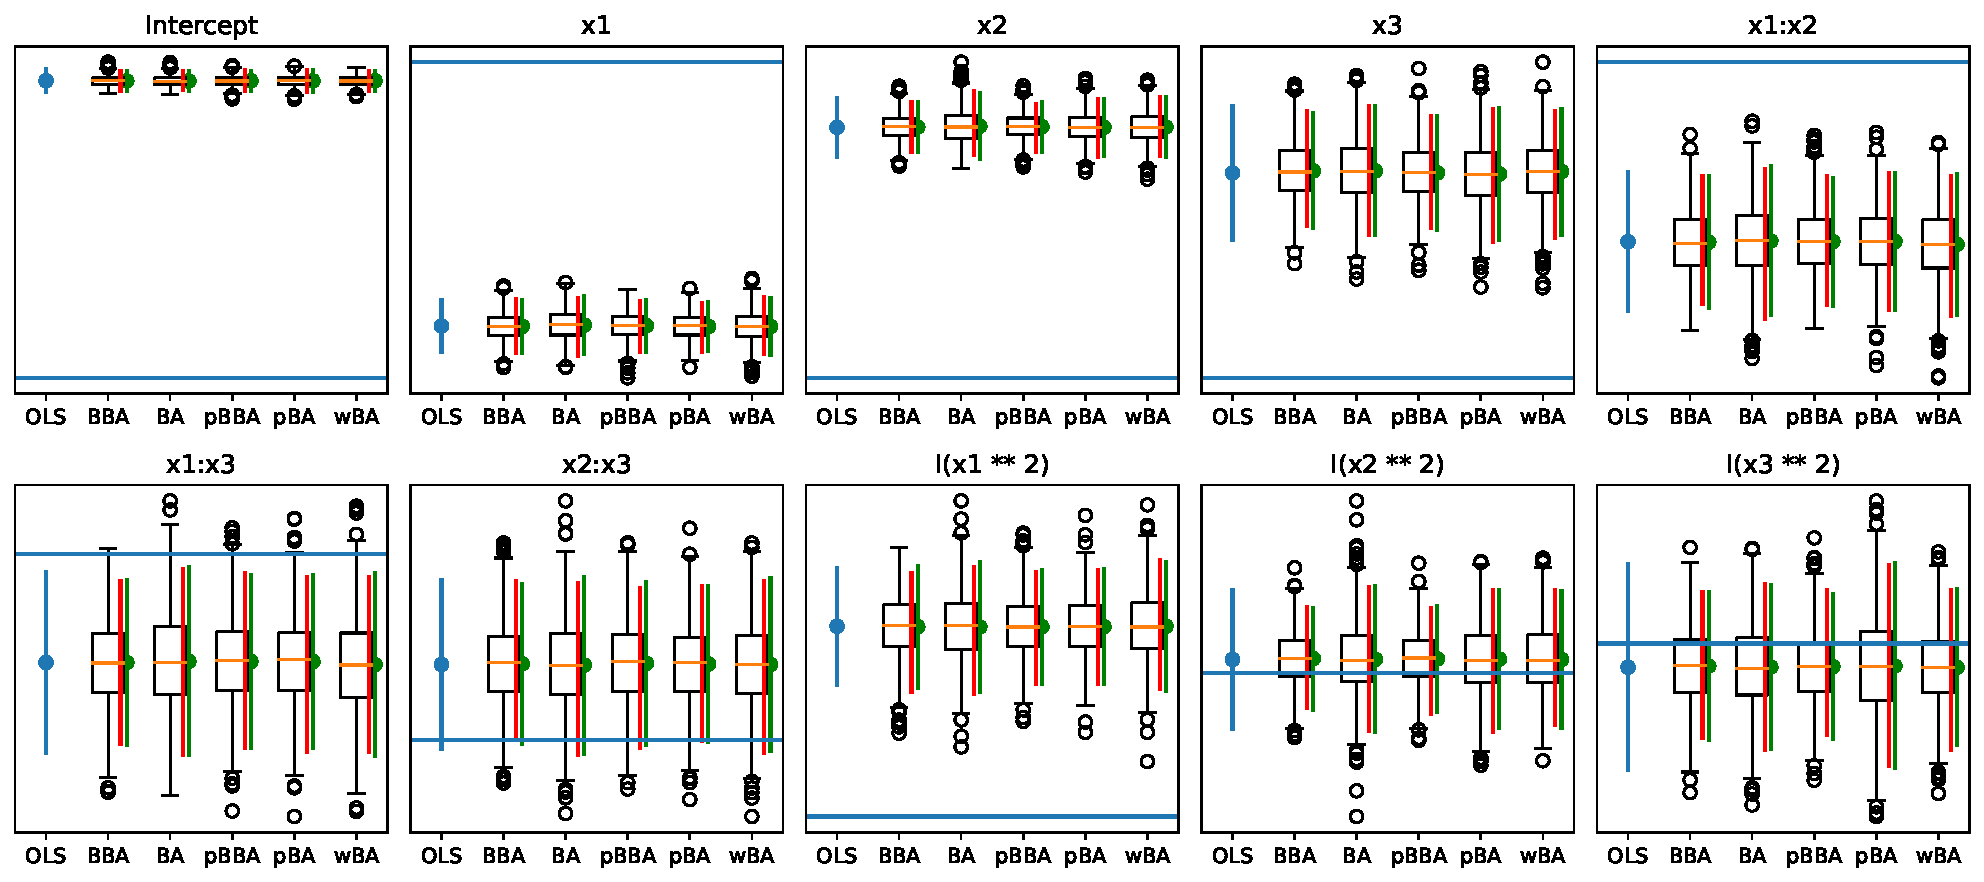
\includegraphics[width=\linewidth]{figures/piston-full-dist.pdf}
    \caption{Distribution of main effects, interactions, and quadratic coefficient estimates for the piston simulation. 
        Blue: ols estimate $\pm$ std.dev. 
        For each bootstrap approach, boxplot: distribution, red: interquartile range, green: mean $\pm$ std.dev.}
    \label{fig:piston-full-dist}
\end{figure}


\subsection{Main effects}
\begin{itemize}
    \item Formula: $seconds \sim x1 + x2 + x3 + x4$
    \item Number of bootstrap samples: 100
    \item Distribution of bootstrap sampled coefficients: Figure~\ref{fig:piston-main-dist}
\end{itemize}

\subsection{Interactions}
\begin{itemize}
    \item Formula: $seconds \sim x1 + x2 + x3 + x1:x2 + x1:x3 + x2:x3$
    \item Number of bootstrap samples: 100
    \item Distribution of bootstrap sampled coefficients: Figure~\ref{fig:piston-int-dist}
\end{itemize}

\subsection{Quadratic model}
\begin{itemize}
    \item Formula: $seconds \sim x1 + x2 + x3 + x1^2 + x2^2 + x3^2$
    \item Number of bootstrap samples: 100
    \item Distribution of bootstrap sampled coefficients: Figure~\ref{fig:piston-quadratic-dist}
\end{itemize}

\subsection{Full model}
\begin{itemize}
    \item Formula: $seconds \sim x1 + x2 + x3 + x1:x2 + x1:x3 + x2:x3 + x1^2 + x2^2 + x3^2$
    \item Number of bootstrap samples: 100
    \item Distribution of bootstrap sampled coefficients: Figure~\ref{fig:piston-full-dist}
\end{itemize}

\subsection{Comparisons}

\begin{table}
\centering
\caption{BBA std. deviation of the regression coefficients for the Piston simulation.}
\label{tbl:piston-BBA}
\begin{adjustbox}{angle=90}\begin{tabular}{lrrrrrrrrrrrrrrrrrr}
\toprule
 & \multicolumn{3}{c}{Main} & \multicolumn{3}{c}{Full} \\
 & Regr. & BBA & Delta & Regr. & BBA & Delta \\
\midrule
Intercept & \red{0.82342} & \red{0.60483} & \red{-26.5} & \red{1.19664} & \red{1.03030} & \red{-13.9} \\
x1 & \red{0.95080} & \red{0.76040} & \red{-20.0} & \red{0.78772} & \red{0.80110} & \red{1.7} \\
x2 & \red{0.95080} & \red{0.68112} & \red{-28.4} & \red{0.78772} & \red{0.66288} & \red{-15.8} \\
x3 & \red{0.95080} & \red{0.65951} & \red{-30.6} & \red{0.78772} & \red{0.67731} & \red{-14.0} \\
x4 & 0.95080 & 0.63040 & -33.7 &  &  &  \\
x1:x2 &  &  &  & \red{0.96476} & \red{0.92408} & \red{-4.2} \\
x1:x3 &  &  &  & \red{0.96476} & \red{0.88620} & \red{-8.1} \\
x2:x3 &  &  &  & \red{0.96476} & \red{0.91043} & \red{-5.6} \\
I(x1 ** 2) &  &  &  & \red{0.70794} & \red{0.73775} & \red{4.2} \\
I(x2 ** 2) &  &  &  & 0.70794 & 0.51710 & -27.0 \\
I(x3 ** 2) &  &  &  & 0.70794 & 0.50657 & -28.4 \\
\bottomrule
\end{tabular}\end{adjustbox}
\end{table}

\begin{table}
\centering
\caption{BA std. deviation of the regression coefficients for the Piston simulation.}
\label{tbl:piston-BA}
\begin{adjustbox}{angle=90}\begin{tabular}{lrrrrrrrrrrrrrrrrrr}
\toprule
 & \multicolumn{3}{c}{Main} & \multicolumn{3}{c}{Full} \\
 & Regr. & BA & Delta & Regr. & BA & Delta \\
\midrule
Intercept & \red{0.82342} & \red{0.80394} & \red{-2.4} & \red{1.19664} & \red{1.03789} & \red{-13.3} \\
x1 & \red{0.95080} & \red{1.18924} & \red{25.1} & \red{0.78772} & \red{0.87550} & \red{11.1} \\
x2 & \red{0.95080} & \red{0.94900} & \red{-0.2} & \red{0.78772} & \red{0.87109} & \red{10.6} \\
x3 & \red{0.95080} & \red{0.93570} & \red{-1.6} & \red{0.78772} & \red{0.76117} & \red{-3.4} \\
x4 & 0.95080 & 0.85582 & -10.0 &  &  &  \\
x1:x2 &  &  &  & \red{0.96476} & \red{1.03973} & \red{7.8} \\
x1:x3 &  &  &  & \red{0.96476} & \red{1.00755} & \red{4.4} \\
x2:x3 &  &  &  & \red{0.96476} & \red{1.00718} & \red{4.4} \\
I(x1 ** 2) &  &  &  & \red{0.70794} & \red{0.78125} & \red{10.4} \\
I(x2 ** 2) &  &  &  & 0.70794 & 0.74039 & 4.6 \\
I(x3 ** 2) &  &  &  & 0.70794 & 0.56505 & -20.2 \\
\bottomrule
\end{tabular}\end{adjustbox}
\end{table}

\begin{table}
\centering
\caption{pBBA std. deviation of the regression coefficients for the Piston simulation.}
\label{tbl:piston-pBBA}
\begin{adjustbox}{angle=90}\begin{tabular}{lrrrrrrrrrrrrrrrrrr}
\toprule
 & \multicolumn{3}{c}{Main} & \multicolumn{3}{c}{Full} \\
 & Regr. & pBBA & Delta & Regr. & pBBA & Delta \\
\midrule
Intercept & \red{0.82342} & \red{0.60831} & \red{-26.1} & \red{1.19664} & \red{1.04301} & \red{-12.8} \\
x1 & \red{0.95080} & \red{0.77756} & \red{-18.2} & \red{0.78772} & \red{0.77756} & \red{-1.3} \\
x2 & \red{0.95080} & \red{0.66149} & \red{-30.4} & \red{0.78772} & \red{0.66149} & \red{-16.0} \\
x3 & \red{0.95080} & \red{0.66926} & \red{-29.6} & \red{0.78772} & \red{0.66926} & \red{-15.0} \\
x4 & 0.95080 & 0.64859 & -31.8 &  &  &  \\
x1:x2 &  &  &  & \red{0.96476} & \red{0.89139} & \red{-7.6} \\
x1:x3 &  &  &  & \red{0.96476} & \red{0.92286} & \red{-4.3} \\
x2:x3 &  &  &  & \red{0.96476} & \red{0.92514} & \red{-4.1} \\
I(x1 ** 2) &  &  &  & \red{0.70794} & \red{0.69214} & \red{-2.2} \\
I(x2 ** 2) &  &  &  & 0.70794 & 0.54135 & -23.5 \\
I(x3 ** 2) &  &  &  & 0.70794 & 0.50015 & -29.4 \\
\bottomrule
\end{tabular}\end{adjustbox}
\end{table}

\begin{table}
\centering
\caption{pBA std. deviation of the regression coefficients for the Piston simulation.}
\label{tbl:piston-pBA}
\begin{adjustbox}{angle=90}\begin{tabular}{lrrrrrrrrrrrrrrrrrr}
\toprule
 & \multicolumn{3}{c}{Main} & \multicolumn{3}{c}{Full} \\
 & Regr. & pBA & Delta & Regr. & pBA & Delta \\
\midrule
Intercept & \red{0.82342} & \red{0.77803} & \red{-5.5} & \red{1.19664} & \red{1.11645} & \red{-6.7} \\
x1 & \red{0.95080} & \red{0.93016} & \red{-2.2} & \red{0.78772} & \red{0.73997} & \red{-6.1} \\
x2 & \red{0.95080} & \red{0.94416} & \red{-0.7} & \red{0.78772} & \red{0.75939} & \red{-3.6} \\
x3 & \red{0.95080} & \red{0.92727} & \red{-2.5} & \red{0.78772} & \red{0.77580} & \red{-1.5} \\
x4 & 0.95080 & 0.93728 & -1.4 &  &  &  \\
x1:x2 &  &  &  & \red{0.96476} & \red{0.95261} & \red{-1.3} \\
x1:x3 &  &  &  & \red{0.96476} & \red{0.92190} & \red{-4.4} \\
x2:x3 &  &  &  & \red{0.96476} & \red{0.89047} & \red{-7.7} \\
I(x1 ** 2) &  &  &  & \red{0.70794} & \red{0.69731} & \red{-1.5} \\
I(x2 ** 2) &  &  &  & 0.70794 & 0.69909 & -1.2 \\
I(x3 ** 2) &  &  &  & 0.70794 & 0.70454 & -0.5 \\
\bottomrule
\end{tabular}\end{adjustbox}
\end{table}

\begin{table}
\centering
\caption{wBA std. deviation of the regression coefficients for the Piston simulation.}
\label{tbl:piston-wBA}
\begin{adjustbox}{angle=90}\begin{tabular}{lrrrrrrrrrrrrrrrrrr}
\toprule
 & \multicolumn{3}{c}{Main} & \multicolumn{3}{c}{Full} \\
 & Regr. & wBA & Delta & Regr. & wBA & Delta \\
\midrule
Intercept & \red{0.82342} & \red{0.82554} & \red{0.3} & \red{1.19664} & \red{1.04128} & \red{-13.0} \\
x1 & \red{0.95080} & \red{1.17701} & \red{23.8} & \red{0.78772} & \red{0.85080} & \red{8.0} \\
x2 & \red{0.95080} & \red{0.91483} & \red{-3.8} & \red{0.78772} & \red{0.80444} & \red{2.1} \\
x3 & \red{0.95080} & \red{0.86632} & \red{-8.9} & \red{0.78772} & \red{0.74086} & \red{-5.9} \\
x4 & 0.95080 & 0.85109 & -10.5 &  &  &  \\
x1:x2 &  &  &  & \red{0.96476} & \red{0.98511} & \red{2.1} \\
x1:x3 &  &  &  & \red{0.96476} & \red{0.97772} & \red{1.3} \\
x2:x3 &  &  &  & \red{0.96476} & \red{0.97938} & \red{1.5} \\
I(x1 ** 2) &  &  &  & \red{0.70794} & \red{0.77889} & \red{10.0} \\
I(x2 ** 2) &  &  &  & 0.70794 & 0.69552 & -1.8 \\
I(x3 ** 2) &  &  &  & 0.70794 & 0.53633 & -24.2 \\
\bottomrule
\end{tabular}\end{adjustbox}
\end{table}



\end{document}
